% !TeX root = ../main.tex
\documentclass[./../main.tex]{subfiles}

\begin{document}

\section{Phân tích yêu cầu}
Như đã đề cập ở các phần trước, mục tiêu hướng đến của đề tài là xây dựng một phần mềm theo dõi sắn với nhiều tính năng bao gồm xem các bảng dữ liệu về sắn, bệnh trên cây sắn, bản đồ dịch bệnh, chẩn đoán bệnh, xem danh sách nguồn cung, thêm, sửa, xóa các đề xuất thương mại sắn và xem, viết các bài báo. Do đó, hệ thống phải đáp ứng được khả năng quản lý nhiều dữ liệu, cũng như đảm bảo cho cả người dùng và quản trị viên có thể thao tác thuận tiện. Ngoài ra còn có thêm một số chức năng phát triển thêm để phần mềm được hoàn thiện hơn như đăng ký, đăng nhập, quên mật khẩu, chỉnh sửa thông tin cá nhân để người dùng có thể sử dụng với đúng vai trò tương ứng, đảm bảo tính bảo mật, an toàn. Dự án này được phát triển từ bài toán do Viện Khoa học \& công nghệ Việt Nam - Hàn Quốc (VKIST) đề ra, và nhu cầu thực tiễn của người nông dân trồng sắn hay những người có liên quan đến ngành nông nghiệp này; vậy nên, việc chú trọng vào UI/UX cũng như thiết kế cơ sở dữ liệu sao cho hợp lý, tiết kiệm chi phí là điều cần thiết. Dựa vào những điều trên, sau đây sẽ đi vào phần phân tích vấn đề thành các yêu cầu, các ca sử dụng.

\subsection{Đặc tả yêu cầu chức năng}
Chia hệ thống thành các nhóm chức năng chính theo mối liên hệ lẫn nhau giữa các chức năng và sự tương đồng trong cách sử dụng, cách thực thi của chúng sẽ thu được các đặc tả yêu cầu của nhóm chức năng. Dựa vào các đặc tả này để phân tích thành các ca sử dụng, đặc tả ca sử dụng, và luồng hoạt động. Có thể phân chia đối tượng sử dụng thành 3 nhóm sau: người dùng là khách chỉ có thể xem và tìm kiếm một số thông tin, người dùng có tài khoản đã được xác minh có thể cung cấp nguồn sắn, giao dịch thương mại sắn, viết bài báo mới; và cuối cùng là quản trị viên điều hành phần mềm.

\begin{itemize} 
    \item \textbf{Quản lý tài khoản:} Người dùng khách có thể đăng ký tạo tài khoản. Sau khi tài khoản được quả trị viên duyệt thì có thể dùng tài khoản đó để đăng nhập, sửa lại thông tin cá nhân và các dữ liệu liên quan đến tài khoản đó trên sàn thương mại. Khi muốn kết thúc phiên đăng nhập thì cần đăng xuất khỏi hệ thống.
    \item \textbf{Tổng hợp thông tin về sắn, bệnh trên cây sắn:} Hiển thị tổng hợp các thống tin về sắn, bệnh trên cây sắn, dưới dạng bảng giúp người dùng dễ dàng nắm bắt thông tin. Có thể tìm theo tên hoặc nhãn, xem chi tiết thông tin sắn hoặc bệnh trên cây sắn nhắm mục đích tiết kiệm thời gian trong việc tìm kiếm thông tin theo nhu cầu cá nhân.
    \item \textbf{Bản đồ sắn:} Hiển thị bản đồ Tây Ninh với các điểm được đánh dấu nơi diễn ra dịch bệnh và thông tin về dịch bệnh đó. Ngoài ra cũng hộ trợ người dùng truy vấn thông tin về dịch bệnh theo khu vực, loại bệnh, mức độ nghiêm trọng của dịch bệnh để họ có thể kịp thời ứng phó và tìm cách phòng chống, chữa trị nếu mắc phải.
    \item \textbf{Chẩn đoán bệnh bằng hình ảnh:} Để chẩn đoán bệnh trên cây sắn, người dùng sau khi tải ảnh lên, hệ thống sẽ trả về kết quả xác suất bệnh trên cây sắn được phân tích từ ảnh. Về phần cách để chẩn đoán bệnh, hệ thống sẽ gửi ảnh cho bên thứ ba qua API và đợi kết quả trả về để hiển thị, nên cách phân tích bệnh qua ảnh sẽ không được trình bày cụ thể trong khóa luận tốt nghiệp này.
    \item \textbf{Danh sách nguồn cung sắn:} Danh sách các tài khoản đã được xác minh và có thể cung cấp nguồn sắn dưới dạnh bảng với chức năng có thể tìm kiếm những nhà cung cấp tùy theo yêu cầu người dùng.
    \item \textbf{Thương mại sắn:} Khi đăng nhập vào hệ thống bằng tài khoản đã được xác minh, người dùng có thể theo dõi các hoạt động thương mại về mua, bán sắn, người dùng cũng có thể tham gia tạo đề xuất trao đổi sắn và quản lý các đề xuất đó như thêm giống sắn, gia hạn thêm thời gian giao dịch.
    \item \textbf{Diễn đàn:} Trong khi khách chỉ có thể xem các bài báo công khai trên trang phần mềm, thì người dùng đã được xác minh khi đăng nhập có thể thêm mới các bài viết liên quan đến sắn. Khi đăng bài báo mới, người dùng cần đảm bảo tính đúng đắn và pháp lý, bản quyền của bài báo đó.
    \item \textbf{Quản lý phần mềm đối với quản trị viên:} Quản trị viên có thể quản lý dữ liệu của toàn bộ hệ thống, cụ thể là: dữ liệu về các giống sắn, bệnh trên cây sắn, bản đồ dịch bệnh mà cây sắn mắc phải tại tỉnh Tây Ninh, quản lý diễn đàn sắn, và quản lý tài khoản người dùng, xác minh các tài khoản mới.
\end{itemize}

\subsection{Đặc tả yêu cầu phi chức năng}
Dựa vào bài toán đã được xác định trong phần mở đầu, kết hợp với việc phân tích trải nghiệm người dùng, và các tiêu chuẩn dành cho một trang web như tính khả dụng, tính ổn định, tính bảo mật, hiệu năng hoạt động, khả năng bảo trì để đưa ra các yêu cầu phi chức năng. Đây cũng là cơ sở cho việc kiểm thử hệ thống sau này có đáp ứng được các yêu cầu này không, từ đó đưa ra đánh giá và hướng giải quyết.

\subsubsection{Tính khả dụng}
\begin{enumerate}
    \item Giao diện cần có sự thống nhất về bố cục và thân thiên với người dùng, nội dung được hiển thị trực quan, phù hợp với chủ đề chung của phần mềm. Đáp ứng các đối tượng người dùng đã xác định trước đó.
    \item Có thể hiển thị các giao diện, bố cục khác nhau tùy thuộc vào thiết bị điện tử mà người dùng sử dụng, từ máy tính xách tay, máy tính bảng đến các thiết bị nhỏ hơn như điện thoại thông minh, hỗ trợ các trình duyệt web phổ biến như Google Chrome, Microsoft Edge, Samsung Internet,... Để việc trình bày giao diện đạt hiệu quả tốt nhất, khuyến khích người sử dụng dùng trình duyệt Google Chrome trên máy tính xách tay hay máy cây.
\end{enumerate}

\subsubsection{Tính ổn định của hệ thống}
\begin{enumerate}
    \item Trong trường hợp hệ thống xảy ra các sự cố và ngừng vận hành, bị đóng băng, thì cần nhanh chóng khắc phục lỗi và phục hồi lại bằng cách tải lại frontend, backend. Nếu không khắc phục được, cần tiến hành tải lại phiên bản cũ vận hành được và kiểm tra nguyên nhân gây lỗi để sửa đổi kịp thời.
    \item Những lỗi chấp nhận được là lỗi không gây tổn hại trầm trọng cho hệ thống và có thể khắc phục hoàn toàn trong 24 giờ, thường là những lỗi về giao diện, không tác động tới cơ sở dữ liệu. Với những lỗi như vậy cần nhanh chóng tìm và sửa để tránh cho việc trải nghiệm người dùng bị ảnh hưởng.
\end{enumerate}

\subsubsection{Tính bảo mật của hệ thống}
\begin{enumerate}
    \item Đảm báo phân quyền cho các đối tượng đúng thẩm quyền, giới hạn các chức năng có thể sử dụng ở cả frontend và backend theo đối tượng sử dụng. Nhờ đó, các tác nhân sẽ chỉ có thể và chỉ tập trung vào các chức năng mà họ có thể sử dụng, tránh việc nhầm lẫn có thể ảnh hưởng tới dữ liệu hệ thống.
    \item Một số chức năng đặc thù dành riêng có người dùng có tài khoản đã xác minh như quản lý đề xuất sắn và viết bài báo mới, đều sẽ tác động đến cơ sở dữ liệu, đều cần phải thông qua tài khoản đã đăng nhập và gửi yêu cầu bằng token còn hiệu lực. Từ đó tránh được việc tạo ra các thông tin giả, gây nhiễu loạn thông tin cho người dùng khác. Việc xác minh tài khoản cũng giúp cho quản trị viên có thể liên lạc tới người dùng khi trong trường hợp gặp sự cố.
\end{enumerate}

\subsubsection{Hiệu năng hoạt động}
\begin{enumerate}
    \item Phần mềm cần hoạt động liên tục, hạn chế việc thời gian chết trong quá trình cài đặt phần mềm trên máy chủ ảo. Đảm bảo đáp ứng được các yêu cầu từ người dùng lên tới 100 người dùng cùng lúc và thời gian phản hồi là dưới 1 giây.
    \item Vì đặc thù của phần mềm là những người nông dân trồng sắn hay các cá nhân, tổ chức có liên quan đến loại cây này, nên mức độ tăng trưởng và mở rộng của phần mềm là không cao, tuy nhân kì vọng là có thể đạt được 10 người đăng ký mới mỗi tháng. Để đạt được mục tiêu thì ngoài việc duy trì hệ thống không bị gián đoạn thì còn cần thường xuyên cập nhật các chức năng mới thu hút người dùng.
\end{enumerate}

\subsubsection{Tính bảo trì của hệ thống}
\begin{enumerate}
    \item Cần sao lưu lại dữ liệu của hệ thống phòng trường hợp các sự cố như bị tấn công hay máy chủ gặp vấn đề gây mất mát dữ liệu. Nhờ đó có thể nhanh chóng phục hồi dữ liệu và tiếp tục vận hành hệ thống.
    \item Nếu gặp vấn đề trong phiên bản mới vừa cập nhật trên máy chủ, cần phải đảm bảo có thể quay trở lại phiên bản trước và sửa lỗi kịp thời, tránh làm ảnh hưởng người dùng. Phần mềm có thể cài đặt và quản lý dễ dàng bằng việc ứng dụng Github trong quản lý các phiên bản phần mềm và Docker trong việc cài đặt hệ thống.
\end{enumerate}


Đáp ứng > 90\% trên toàn bộ mẫu người dùng:
\begin{itemize}
    \item Học cách sử dụng hệ thống trong < 5 phút.
    \item Đăng ký, đăng nhập < 1 phút.
    \item Tìm kiếm các thông tin ở các trang tương ứng < 1 phút.
    \item Đáp ứng thời gian vận hành liên tục trên 98\%.
\end{itemize}

\subsubsection{Hiệu suất}
\begin{itemize}
	\item Đáp ứng ít nhất cho 1.000 CCU.
	\item Đáp ứng 99\% số yêu cầu dưới 2s.
	\item Trung bình thời gian phản hồi mỗi yêu cầu là dưới 2s.
\end{itemize}

\subsubsection{Bảo mật}
\begin{itemize}
	\item Khả năng bảo vệ hệ thống trước tấn công DDoS hạn chế các lỗ hổng nguy hiểm.
	\item Bảo mật về thông tin cá nhân.
\end{itemize}

\subsection{Giả định và ràng buộc}
\begin{itemize}
    \item \textbf{Công nghệ sử dụng}: Ứng dụng CRUD (Create READ Update Delete) bằng các công nghệ: ReactJS, Directus.
    \item \textbf{Chi phí}: Hầu như không mất phí.
    \item \textbf{Thời gian phát triển}: Nhỏ hơn 6 tháng.
    \item \textbf{Khả năng tương thích}: Có khả năng tương thích với các thiết bị máy tính cây, máy tính cá nhân, máy tính bảng, điện thoại thông minh khác nhau. Giao diện tốt nhất khi sử dụng máy tính cá nhân.
\end{itemize}


\section{Các tác nhân hệ thống}

\begin{figure}[H]
    \centering
    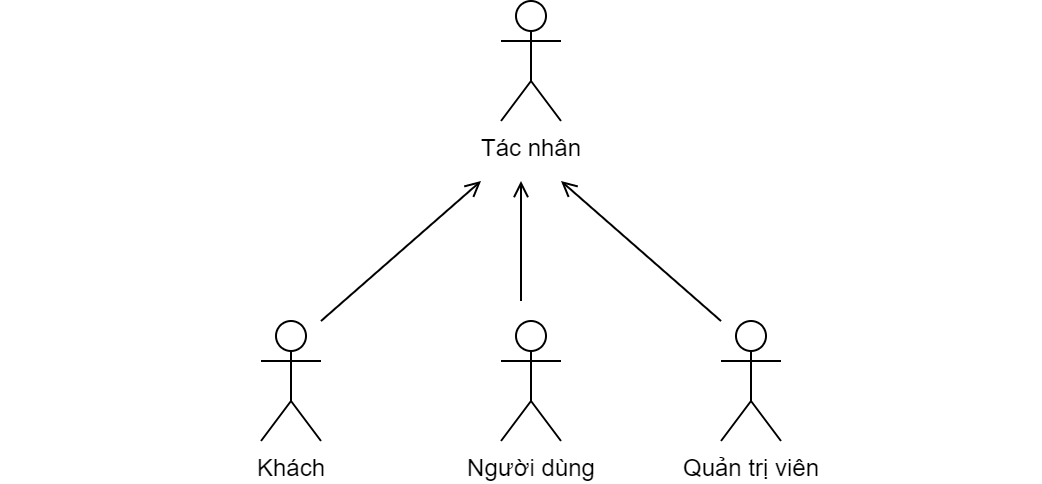
\includegraphics[width=\linewidth]{./img/actors.png}
    \caption{Các tác nhân hệ thống}
\end{figure}

Hệ thống có 3 tác nhân:
\begin{itemize}
    \item \textbf{Khách}: Bất kỳ người dùng nào khi truy cập website đều có thể xem và tra cứu các thông tin mở. Nhóm người này có thể xem và tìm kiếm các thông tin hữu ích liên quan đến sắn.
    \item \textbf{Người dùng}: Người dùng của hệ thống cần phải có tài khoản đã xác nhận. Nhóm người này có thể truy cập vào website và thực hiện các công việc yêu cầu tính xác minh thông tin cá nhân, vậy nên cần phải cung cấp đủ thông tin cũng như cần được quản trị viên duyệt. Một số công việc mà Người dùng có thể thực hiện: thao tác thêm, sửa, xóa đề xuất trên trang thương mại sắn, cập nhật thông tin người dùng,...\
    \item \textbf{Quản trị viên}: Người quản trị toàn bộ cơ sở dữ liệu của hệ thống và Người dùng. Đồng thời cũng là người cập nhật cơ sở dữ liệu, giải quyết các vấn đề của hệ thống. Nhóm người này có thể  là quản trị hệ thống cả về nội dung và con người để đảm bảo hệ thống diễn ra ổn định. Người dùng cần phải được Quản trị viên xác nhận tài khoản để chính thức trở thành Người dùng.
\end{itemize}


\subsection{Đặc tả các ca sử dụng}

Các ca sử dụng:
\begin{figure}[H]
    \centering
    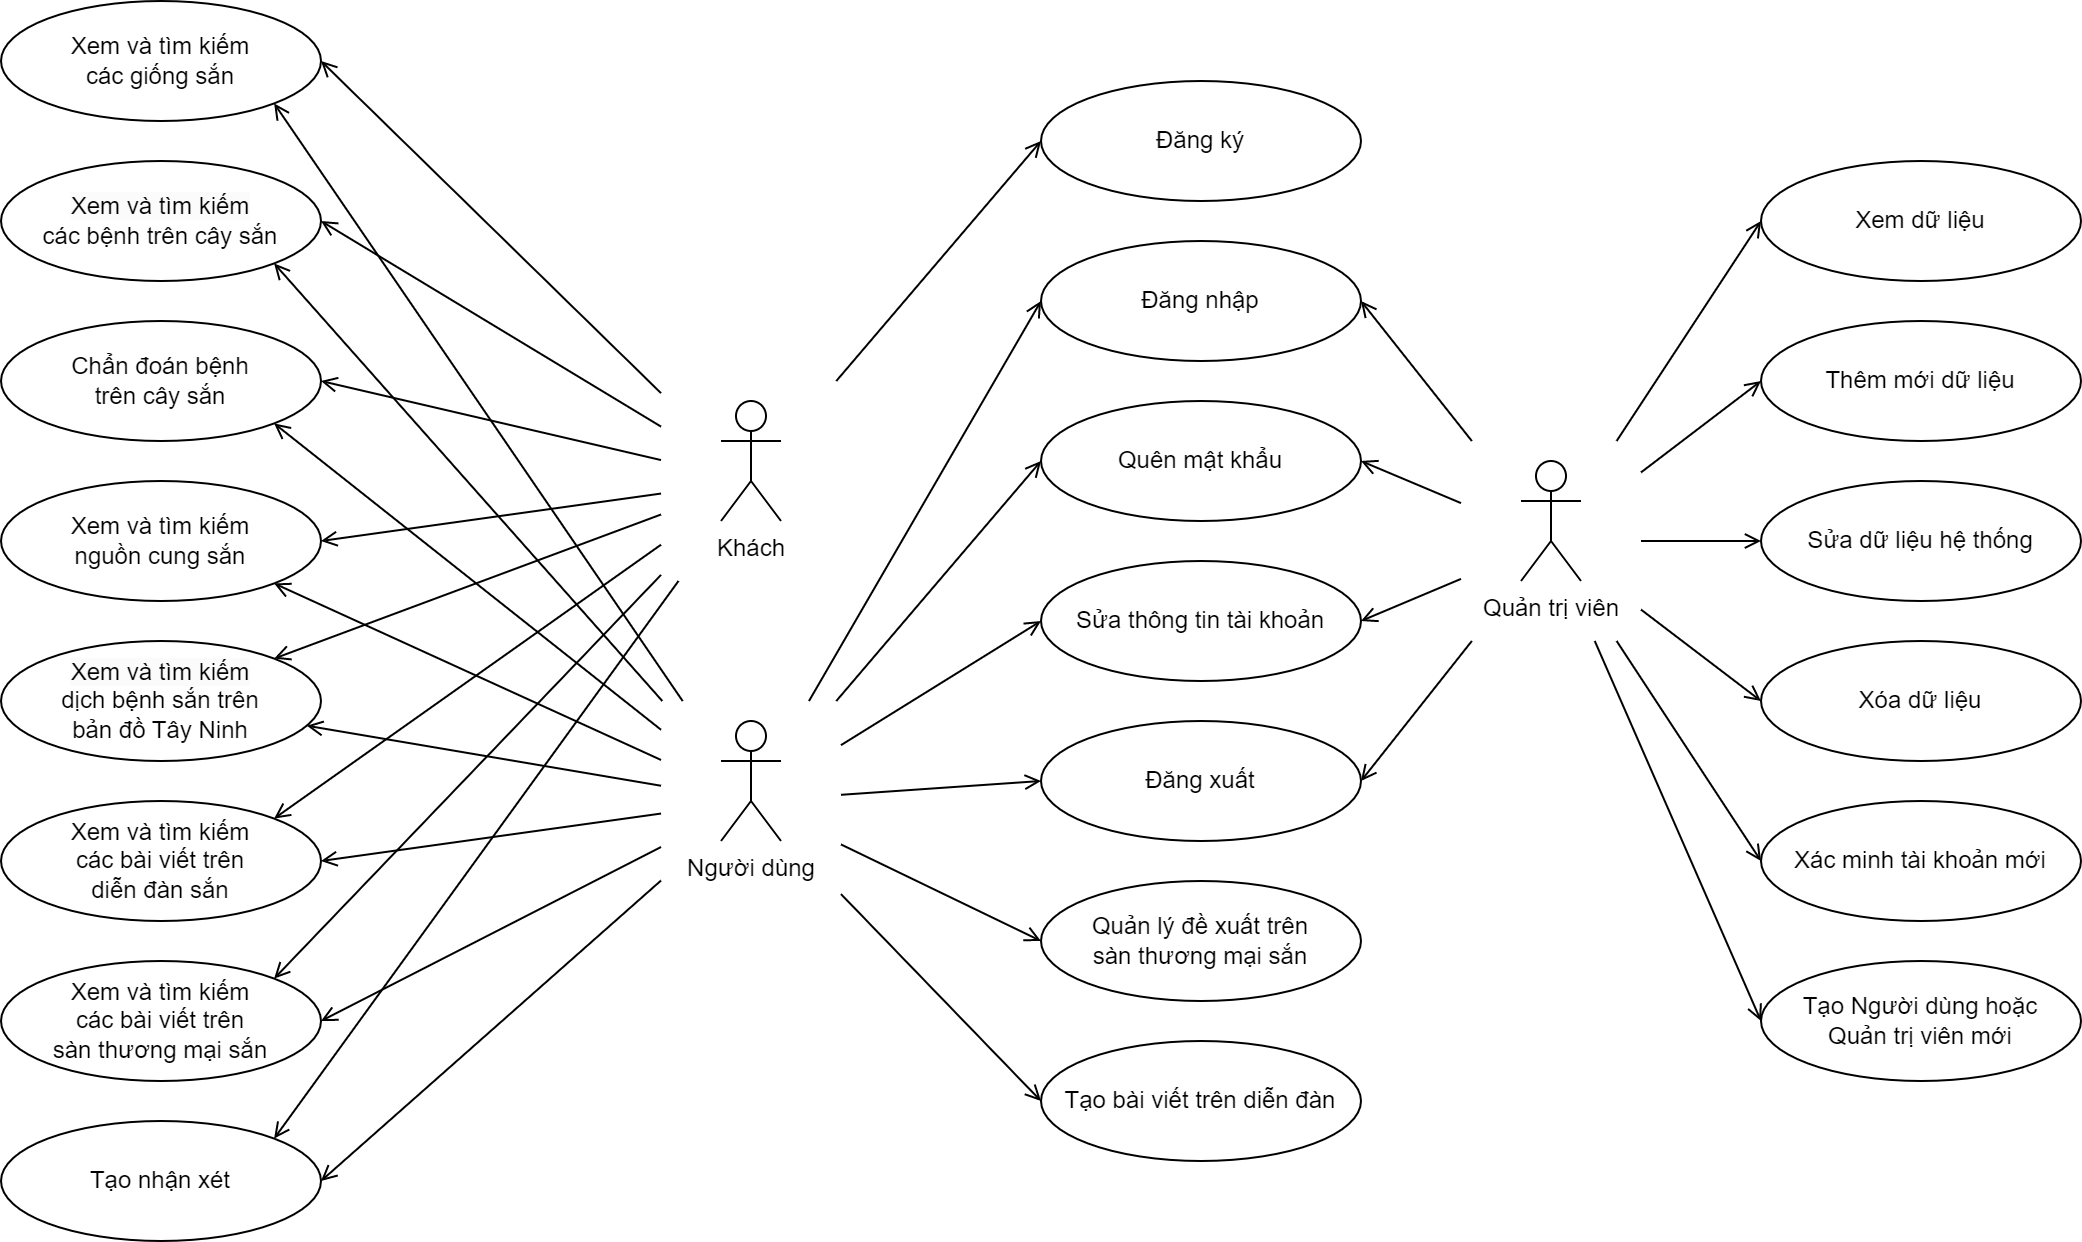
\includegraphics[width=\linewidth]{./img/uc-total.png}
    \caption{Biểu đồ các ca sử dụng}
\end{figure}

Dưới đây sẽ là đặc tả các ca sử dụng:

\subsubsection{Ca sử dụng đăng ký}
\begin{table}[H]
\begin{tabularx}{\textwidth}{| {0.3\textwidth} | X | }
\hline
\textbf{Tên ca sử dụng} & Đăng ký\\ \hline
\textbf{Tác nhân} & Khách\\ \hline
\textbf{Mô tả} & Khách đăng ký làm người dùng của hệ thống.\\ \hline
\textbf{Luồng cơ bản} & \begin{minipage}{0.7\columnwidth}
1. Khách vào trang Đăng nhập và chọn Yêu cầu tạo tài khoản.\\ 2. Hệ thống hiển thị Biểu mẫu đăng ký bao gồm các trường thông tin: email, mật khẩu, nhập lại mật khẩu, tài khoản, họ và tên, số điện thoại.\\ 3. Khách nhập đúng và đủ các trường thông tin cần thiết rồi nhấn nút Gửi yêu cầu.\\ 4. Hệ thống ghi nhận các biểu mẫu hợp lệ và thông báo kết quả Đã gửi yêu cầu thành công. Nếu thông tin không chính xác thì thực hiện luồng thay thế. Nếu chính xác thì tiếp tục.\\ 5. Hệ thống cập nhật thông tin của khách đã gửi yêu cầu tạo tài khoản vào hàng đợi chờ Quản trị viên duyệt.\\
\end{minipage}\\ \hline
\textbf{Luồng thay thế} & \begin{minipage}{0.7\columnwidth}
1. Hệ thống cảnh báo trường thông tin không chính xác bằng cách bôi đỏ trường và hiện gợi ý sửa.\\ 2. Hệ thống yêu cầu khách điền lại dữ liệu.\\ 3. Nếu người dùng đồng ý sửa, điền thêm thông tin thì quay về bước 3 của luồng sự kiện chính, nếu không thì đóng biểu mẫu và kết thúc ca sử dụng.\\
\end{minipage}\\ \hline
\textbf{Tiền điều kiện} & - Không trong trạng thái đã đăng nhập.\\ \hline
\textbf{Hậu điều kiện} & Biểu mẫu yêu cầu tạo tài khoản được thêm vào hàng đợi duyệt.\\ \hline
\end{tabularx}
\end{table}

\subsubsection{Đăng nhập}
\begin{table}[H]
\begin{tabularx}{\textwidth}{| {0.3\textwidth} | X | }
\hline
\textbf{Tên ca sử dụng} & Đăng nhập\\ \hline
\textbf{Tác nhân} & Khách\\ \hline
\textbf{Mô tả} & Khách đăng nhập thành người dùng của hệ thống.\\ \hline
\textbf{Luồng cơ bản} & \begin{minipage}{0.7\columnwidth}
1. Khách vào trang Đăng nhập.\\ 2. Hệ thống hiển thị Biểu mẫu đăng nhập bao gồm hai trường email và mật khẩu.\\ 3. Khách nhập đúng và đủ các trường thông tin cần thiết rồi nhấn nút Gửi yêu cầu.\\ 4. Hệ thống ghi nhận biểu mẫu đã điền đủ hai trường và gửi yêu cầu xác thực. Nếu thông tin không chính xác thì thực hiện luồng thay thế. Nếu chính xác thì tiếp tục.\\ 5. Hệ thống thông báo đăng nhập thành công, khách trở thành người dùng.\\
\end{minipage}\\ \hline
\textbf{Luồng thay thế} & \begin{minipage}{0.7\columnwidth}
- Luồng thay thế a: 1. Hệ thống cảnh báo trường thông tin đã nhập chưa chính xác bằng cách bôi đỏ trường và hiện gợi ý sửa. \\ - Luồng thay thế b: 1. Hệ thống thông báo xác thực email và mật khẩu không thành công.\\ 2. Hệ thống yêu cầu khách điền lại dữ liệu.\\ 3. Nếu người dùng đồng ý sửa, điền thêm thông tin thì quay về bước 3 của luồng sự kiện chính, nếu không thì đóng biểu mẫu và kết thúc ca sử dụng.\\
\end{minipage}\\ \hline
\textbf{Tiền điều kiện} & \begin{minipage}{0.7\columnwidth}
- Không trong trạng thái đã đăng nhập.\\
- Đã gửi yêu cầu tạo tài khoản.\\
\end{minipage}\\ \hline
\textbf{Hậu điều kiện} & Khách đăng nhập thành công thành người dùng hệ thống.\\ \hline
\end{tabularx}
\end{table}

\subsubsection{Quên mật khẩu}
\begin{table}[H]
\begin{tabularx}{\textwidth}{| {0.3\textwidth} | X | }
\hline
\textbf{Tên ca sử dụng} & Quên mật khẩu\\ \hline
\textbf{Tác nhân} & Người dùng\\ \hline
\textbf{Mô tả} & Người dùng quên mật khẩu đăng nhập.\\ \hline
\textbf{Luồng cơ bản} & \begin{minipage}{0.7\columnwidth}
1. Người dùng vào trang Đăng nhập và bấm chọn Quên mật khẩu.\\ 2. Hệ thống hiển thị Biểu mẫu quên mật khẩu gồm duy nhất trường email.\\ 3. Khách nhập đúng email đã đăng ký với hệ thống và bấm nút Gửi.\\ 4. Hệ thống ghi nhận yêu cầu và gửi thư điện tử đến email trên. Nếu email trên chưa có tài khoản tương ứng thì thực hiện luồng thay thế a. Nếu gửi thư điện tử thành công thì tiếp tục.\\ 5. Hệ thống thông báo đăng gửi thư thành công, người dùng kiểm tra thư điện tử và điền biểu mẫu đổi mật khẩu gồm hai trường mật khẩu và nhập lại mật khẩu.\\ 6.  Sau khi người dùng điền đúng định dạng cả hai trường thì bấm Cập nhật mật khẩu. Nếu không muốn thay đổi mật khẩu thì thực hiện luồng thay thế b.\\ 7. Khi mật khẩu thay đổi thành công, hệ thống sẽ thông báo cập nhật thành công tới người dùng và kết thúc ca sử dụng.\\
\end{minipage}\\ \hline
\textbf{Luồng thay thế} & \begin{minipage}{0.7\columnwidth}
- Luồng thay thế a:\\ 1. Hệ thống cảnh báo email đã nhập chưa tồn tại trong hệ thống, lỗi gửi yêu cầu.\\ 2. Hệ thống yêu cầu khách điền lại dữ liệu.\\ 3. Nếu người dùng đồng ý sửa, điền thêm thông tin thì quay về bước 3 của luồng sự kiện chính, nếu không thì đóng biểu mẫu và kết thúc ca sử dụng.\\ - Luồng thay thế b: Người dùng bấm về trang chủ nếu không muốn đổi mật khẩu và kết thúc ca sử dụng.\\
\end{minipage}\\ \hline
\textbf{Tiền điều kiện} & \begin{minipage}{0.7\columnwidth}
- Không trong trạng thái đã đăng nhập.\\ - Đã có tài khoản.\\
\end{minipage}\\ \hline
\textbf{Hậu điều kiện} & Người dùng đổi mật khẩu thành công\\ \hline
\end{tabularx}
\end{table}

\subsubsection{Sửa thông tin tài khoản}
\begin{table}[H]
\begin{tabularx}{\textwidth}{| {0.3\textwidth} | X | }
\hline
\textbf{Tên ca sử dụng} & Sửa thông tin tài khoản\\ \hline
\textbf{Tác nhân} & Người dùng\\ \hline
\textbf{Mô tả} & Người dùng muốn thay đổi thông tin tài khoản.\\ \hline
\textbf{Luồng cơ bản} & \begin{minipage}{0.7\columnwidth}
1. Người dùng vào trang Cá nhân.\\ 2. Hệ thống hiển thị Biểu mẫu đã được khóa, gồm các trường thông tin bao gồm họ và tên, số điện thoại, email, tài khoản, địa chỉ, các giống sắn đang cung cấp, các giống sắn ngừng cung cấp, thông tin chi tiết, mật khẩu mới, nhập lại mật khẩu mới trong trường hợp muốn thay đổi mật khẩu.\\ 3. Người dùng chọn chỉnh sửa trang cá nhân để mở khóa biểu mẫu.\\ 4. Sau khi điền các trường thông tin muốn sửa đúng yêu cầu thì bấm lưu thay đổi hoặc thực hiện luồng thay thế a.\\ 5. Hệ thống thông báo cập nhật thành công và kết thúc ca sử dụng hoặc thực hiện luồng thay thế b.\\
\end{minipage}\\ \hline
\textbf{Luồng thay thế} & \begin{minipage}{0.7\columnwidth}
- Luồng thay thế a:\\ 1. Hệ thống cảnh báo trường thông tin không chính xác bằng cách bôi đỏ trường và hiện gợi ý sửa.\\ 2. Hệ thống yêu cầu khách điền lại dữ liệu.\\ 3. Nếu người dùng đồng ý sửa, điền thêm thông tin thì quay về bước 3 của luồng sự kiện chính, nếu không thì đóng biểu mẫu và kết thúc ca sử dụng.\\ - Luồng thay thế b: Người dùng bấm hủy thay đổi nếu không muốn cập nhật và kết thúc ca sử dụng.\\
\end{minipage}\\ \hline
\textbf{Tiền điều kiện} & - Người dùng đã được xác thực đã đăng nhập.\\ \hline
\textbf{Hậu điều kiện} & Người dùng cập nhập thông tin thành công.\\ \hline
\end{tabularx}
\end{table}

\subsubsection{Đăng xuất}
\begin{table}[H]
\begin{tabularx}{\textwidth}{| {0.3\textwidth} | X | }
\hline
\textbf{Tên ca sử dụng} & Đăng xuất\\ \hline
\textbf{Tác nhân} & Người dùng \\ \hline
\textbf{Mô tả} & Người dùng muốn đăng xuất khỏi hệ thống.\\ \hline
\textbf{Luồng cơ bản} & \begin{minipage}{0.7\columnwidth}
1. Người dùng bấm Đăng xuất dưới bảng chọn khi di chuột qua Tài khoản trên thanh công tiêu đề.\\ 2. Hệ thống thực hiện đăng xuất hoặc luồng thay thế.\\ 3. Người dùng trở thành khách và kết thúc ca sử dụng.\\
\end{minipage}\\ \hline
\textbf{Luồng thay thế} & \begin{minipage}{0.7\columnwidth}
1. Đăng xuất không thành công, hệ thống báo lỗi.\\ 2. Người dùng thực hiện lại bước 1 của luồng cơ bản hoặc kết thúc ca sử dụng, người dùng không trở thành khách.\\
\end{minipage}\\ \hline
\textbf{Tiền điều kiện} & - Người dùng đã đăng nhập hệ thống.\\ \hline
\textbf{Hậu điều kiện} & Người dùng đăng xuất khỏi hệ thống, trở thành khách.\\ \hline
\end{tabularx}
\end{table}

\subsubsection{Xem và tìm kiếm các giống sắn}
\begin{table}[H]
\begin{tabularx}{\textwidth}{| {0.3\textwidth} | X | }
\hline
\textbf{Tên ca sử dụng} & Xem và tìm kiếm các giống sắn\\ \hline
\textbf{Tác nhân} & Khách, người dùng\\ \hline
\textbf{Mô tả} & Các tác nhân xem thông tin tổng hơp, chi tiết về các giống sắn, tìm kiếm giống sắn theo tên, nhãn, tên gốc, tên loài, họ sắn.\\ \hline
\textbf{Luồng cơ bản} & \begin{minipage}{0.7\columnwidth}
1. Tác nhân vào trang các giông sắn.\\ 2. Hệ thống hiển thị dữ liệu dưới dạng bảng các thông tin: số thứ tự, nhãn, tên gốc, tên chủng giông, năm phát hành, nòi giống, và cột xem chi tiết.\\ 3. Tác nhân chọn xem chi tiết để được chuyển tới trang xem đầy đủ thông tin, bao gồm cả hình ảnh về loại sắn tương ứng.\\ 4. Tác nhân cần tìm kiếm thì nhập từ khóa vào ô tìm kiếm rồi chọn tìm kiếm để hệ thống lọc dữ liệu. Để xóa từ khóa, bấm nút tải lại dữ liệu.\\ 5. Trong trường hợp lọc dữ liệu không có kết quả phù hợp thì thực hiện luồng thay thế.\\ 6. Kết thúc ca sử dụng hoặc lặp lại các bước trên.\\
\end{minipage}\\ \hline
\textbf{Luồng thay thế} & 1. Bảng hiển thị không có kết quả tương ứng với bộ lọc. Tác nhân có thể tải lại dữ liệu hoặc kết thúc ca sử dụng. \\ \hline
\textbf{Tiền điều kiện} & Không có. \\ \hline
\textbf{Hậu điều kiện} & Không có. \\ \hline
\end{tabularx}
\end{table}

\subsubsection{Xem và tìm kiếm các bệnh trên cây sắn}
\begin{table}[H]
\begin{tabularx}{\textwidth}{| {0.3\textwidth} | X | }
\hline
\textbf{Tên ca sử dụng} & Xem và tìm kiếm các bệnh trên cây sắn\\ \hline
\textbf{Tác nhân} & Khách, người dùng\\ \hline
\textbf{Mô tả} & Các tác nhân xem thông tin tổng hơp, chi tiết về các bệnh trên cây sắn, tìm kiếm bệnh theo tên tiếng Anh, tên tiếng Việt, nhãn.\\ \hline
\textbf{Luồng cơ bản} & \begin{minipage}{0.7\columnwidth}
1. Tác nhân vào trang các bệnh trên cây sắn.\\ 2. Hệ thống hiển thị dữ liệu dưới dạng bảng các thông tin: số thứ tự, nhãn, tên, tên tiếng Việt, đặc điểm, ảnh hưởng, cách chữa, và cột xem chi tiết.\\ 3. Tác nhân chọn xem chi tiết để được chuyển tới trang xem đầy đủ thông tin, bao gồm cả hình ảnh về bệnh tương ứng.\\ 4. Tác nhân cần tìm kiếm thì nhập từ khóa vào ô tìm kiếm rồi chọn tìm kiếm để hệ thống lọc dữ liệu. Để xóa từ khóa, bấm nút tải lại dữ liệu.\\ 5. Trong trường hợp lọc dữ liệu không có kết quả phù hợp thì thực hiện luồng thay thế.\\ 6. Kết thúc ca sử dụng hoặc lặp lại các bước trên.\\
\end{minipage}\\ \hline
\textbf{Luồng thay thế} & 1. Bảng hiển thị không có kết quả tương ứng với bộ lọc. Tác nhân có thể tải lại dữ liệu hoặc kết thúc ca sử dụng. \\ \hline
\textbf{Tiền điều kiện} & Không có. \\ \hline
\textbf{Hậu điều kiện} & Không có. \\ \hline
\end{tabularx}
\end{table}

\subsubsection{Xem và tìm kiếm nguồn cung sắn}
\begin{table}[H]
\begin{tabularx}{\textwidth}{| {0.3\textwidth} | X | }
\hline
\textbf{Tên ca sử dụng} & Xem và tìm kiếm nguồn cung sắn\\ \hline
\textbf{Tác nhân} & Khách, người dùng \\ \hline
\textbf{Mô tả} & Các tác nhân xem thông tin tổng hơp về các nguồn cung sắn, tìm kiếm theo tên, số điện thoại, lọc theo trạng thái, lọc theo giống sắn.\\ \hline
\textbf{Luồng cơ bản} & \begin{minipage}{0.7\columnwidth}
1. Tác nhân vào trang danh sách nguồn cung sắn.\\ 2. Hệ thống hiển thị dữ liệu dưới dạng bảng các thông tin: số thứ tự, email, địa chỉ, tên, số điện thoại, các loại giống, mô tả chi tiết.\\ 3. Tác nhân cần tìm kiếm thì nhập từ khóa vào ô tìm kiếm rồi chọn tìm kiếm để hệ thống lọc dữ liệu. Tác nhân cần lọc thì chọn bộ lọc tương ứng để lọc dữ liệu. Có thể áp dụng cả tìm kiếm và bộ lọc. Để xóa từ khóa và bộ lọc, bấm nút tải lại dữ liệu.\\ 4. Trong trường hợp lọc dữ liệu không có kết quả phù hợp thì thực hiện luồng thay thế.\\ 5. Kết thúc ca sử dụng hoặc lặp lại các bước trên.\\
\end{minipage}\\ \hline
\textbf{Luồng thay thế} & 1. Bảng hiển thị không có kết quả tương ứng với bộ lọc. Tác nhân có thể tải lại dữ liệu hoặc kết thúc ca sử dụng. \\ \hline
\textbf{Tiền điều kiện} & Không có. \\ \hline
\textbf{Hậu điều kiện} & Không có. \\ \hline
\end{tabularx}
\end{table}

\subsubsection{Xem và tìm kiếm dịch bệnh sắn trên bản đồ Tây Ninh}
\begin{table}[H]
\begin{tabularx}{\textwidth}{| {0.3\textwidth} | X | }
\hline
\textbf{Tên ca sử dụng} & Xem và tìm kiếm dịch bệnh sắn trên bản đồ Tây Ninh\\ \hline
\textbf{Tác nhân} & Khách, người dùng \\ \hline
\textbf{Mô tả} & Các tác nhân xem thông tin tổng hơp về các vùng đang xảy ra dịch bệnh trên cây sắn trên bản đồ tỉnh Tây Ninh.\\ \hline
\textbf{Luồng cơ bản} & \begin{minipage}{0.7\columnwidth}
1. Tác nhân vào trang bản đồ theo dõi nguồn giống.\\ 2. Hệ thống hiển thị bảng tổng hợp và bản đồ chứa các điểm biểu thị nơi diễn ra dịch bệnh.\\ 3. Tác nhân bấm vào điểm biểu thị để xem thông tin về dịch bệnh tương ứng, gồm các thông tin: tên bệnh, giống sắn đang mắc bệnh, mức độ nghiêm trọng.\\ 4. Tác nhân cần lọc dữ liệu thì chọn bộ lọc sắn, bệnh, mức độ, thành phố/quận, huyện/phường tương ứng để lọc dữ liệu. Để xóa bộ lọc, bấm nút tải lại dữ liệu.\\ 5. Trong trường hợp lọc dữ liệu không có kết quả phù hợp thì thực hiện luồng thay thế.\\ 6. Kết thúc ca sử dụng hoặc lặp lại các bước trên.\\
\end{minipage}\\ \hline
\textbf{Luồng thay thế} & 1. Bảng hiển thị và bản đồ không có kết quả tương ứng với bộ lọc. Tác nhân có thể tải lại dữ liệu hoặc kết thúc ca sử dụng. \\ \hline
\textbf{Tiền điều kiện} & Không có. \\ \hline
\textbf{Hậu điều kiện} & Không có. \\ \hline
\end{tabularx}
\end{table}

\subsubsection{Xem và tìm kiếm các bài viết trên diễn đàn sắn}
\begin{table}[H]
\begin{tabularx}{\textwidth}{| {0.3\textwidth} | X | }
\hline
\textbf{Tên ca sử dụng} & Xem và tìm kiếm các bài viết trên diễn đàn sắn\\ \hline
\textbf{Tác nhân} & Khách, người dùng \\ \hline
\textbf{Mô tả} & Các tác nhân xem thông tin tổng hơp, chi tiết về các bài viết trên diễn đàn sắn, tìm kiếm theo tên, lọc theo thẻ tag.\\ \hline
\textbf{Luồng cơ bản} & \begin{minipage}{0.7\columnwidth}
1. Tác nhân vào trang diễn đàn.\\ 2. Hệ thống hiển thị dữ liệu dưới dạng các thẻ nhỏ chứa một phần nội dung bài viết: ảnh, tên vài viết, thẻ tag, 100 kí tự đầu của bài viết.\\ 3. Tác nhân chọn bài viết muốn xem chi tiết để được chuyển tới trang xem đầy đủ bài viết.\\ 4. Tác nhân cần tìm kiếm thì nhập từ khóa vào ô tìm kiếm rồi chọn tìm kiếm để hệ thống lọc dữ liệu. Tác nhân cần lọc thẻ tag thì chọn bộ lọc tương ứng để lọc dữ liệu. Có thể áp dụng cả tìm kiếm và bộ lọc. Để xóa từ khóa và bộ lọc, bấm nút tải lại dữ liệu.\\ 5. Trong trường hợp lọc dữ liệu không có kết quả phù hợp thì thực hiện luồng thay thế.\\ 6. Kết thúc ca sử dụng hoặc lặp lại các bước trên.\\
\end{minipage}\\ \hline
\textbf{Luồng thay thế} & 1. Trang không có kết quả tương ứng với bộ lọc. Tác nhân có thể tải lại dữ liệu hoặc kết thúc ca sử dụng. \\ \hline
\textbf{Tiền điều kiện} & Không có. \\ \hline
\textbf{Hậu điều kiện} & Không có. \\ \hline
\end{tabularx}
\end{table}

\subsubsection{Xem và tìm kiếm các bài viết trên sàn thương mại sắn}
\begin{table}[H]
\begin{tabularx}{\textwidth}{| {0.3\textwidth} | X | }
\hline
\textbf{Tên ca sử dụng} & Xem và tìm kiếm các bài viết trên sàn thương mại sắn\\ \hline
\textbf{Tác nhân} & Người dùng\\ \hline
\textbf{Mô tả} & Các tác nhân xem thông tin tổng hơp về các đề xuất mua, bán sắn trên sàn thương mại, tìm kiếm theo tên, tiêu đề, số điện thoại, nhãn sắn.\\ \hline
\textbf{Luồng cơ bản} & \begin{minipage}{0.7\columnwidth}
1. Tác nhân vào trang thương mại sắn.\\ 2. Hệ thống hiển thị dữ liệu dưới dạng bảng bao bảng các thông tin: số thứ tự, tiêu đề, họ và tên, số điện thoại, miêu tả, thông tin chi tiết, thời gian bắt đầu - kết thúc. Đề xuất đang trong thời gian hoạt động thì hàng tương ứng có nền màu xanh, ngoài thời gian đó sẽ có nền màu xám.\\ 3. Tác nhân cần tìm kiếm thì nhập từ khóa vào ô tìm kiếm rồi chọn tìm kiếm để hệ thống lọc dữ liệu. Để xóa từ khóa, bấm nút tải lại dữ liệu.\\ 4. Trong trường hợp lọc dữ liệu không có kết quả phù hợp thì thực hiện luồng thay thế.\\ 5. Kết thúc ca sử dụng hoặc lặp lại các bước trên.\\
\end{minipage}\\ \hline
\textbf{Luồng thay thế} & 1. Bảng không có kết quả tương ứng với bộ lọc. Tác nhân có thể tải lại dữ liệu hoặc kết thúc ca sử dụng. \\ \hline
\textbf{Tiền điều kiện} & - Người dùng đã được xác thực đã đăng nhập.\\ \hline
\textbf{Hậu điều kiện} & Không có. \\ \hline
\end{tabularx}
\end{table}

\subsubsection{Chẩn đoán bệnh trên cây sắn}
\begin{table}[H]
\begin{tabularx}{\textwidth}{| {0.3\textwidth} | X | }
\hline
\textbf{Tên ca sử dụng} & Chẩn đoán bệnh trên cây sắn\\ \hline
\textbf{Tác nhân} & Khách, người dùng \\ \hline
\textbf{Mô tả} & Tác nhân tải lên ảnh bệnh trên cây sắn, hệ thống phân tích và trả về kết quả xác suất các bệnh có thể đang mắc phải.\\ \hline
\textbf{Luồng cơ bản} & \begin{minipage}{0.7\columnwidth}
1. Tác nhân vào trang chẩn đoán bệnh.\\ 2. Tác nhân tải lên ảnh bệnh trên cây sắn, hệ thống phân tích từ ảnh xác suất các bệnh có thể xảy ra, rồi trả về bảng kết quả được sắp xếp theo thứ tự xác suất từ cao xuống thấp. \\ 3. Tác nhân có thể lặp lại bước 1 nếu muốn tiếp tục chẩn đoán khác hoặc kết thúc ca sử dụng.
\end{minipage}\\ \hline
\textbf{Luồng thay thế} & Không có. \\ \hline
\textbf{Tiền điều kiện} & Không có. \\ \hline
\textbf{Hậu điều kiện} & Trả ra kết quả chẩn đoán sắp xếp theo xác suất bệnh gần đúng nhất.\\ \hline
\end{tabularx}
\end{table}

\subsubsection{Tạo nhận xét}
\begin{table}[H]
\begin{tabularx}{\textwidth}{| {0.3\textwidth} | X | }
\hline
\textbf{Tên ca sử dụng} & Tạo nhận xét\\ \hline
\textbf{Tác nhân} & Khách, người dùng\\ \hline
\textbf{Mô tả} & Các tác nhân gửi nhận xét về hệ thống.\\ \hline
\textbf{Luồng cơ bản} & \begin{minipage}{0.7\columnwidth}
1. Tác nhân vào trang chủ.\\ 2. Hệ thống hiển thị biểu mẫu gồm tên, email, nhận xét về hệ thống, tác nhân điền đúng và đủ thông tin rồi bấm gửi.\\ 3. Hệ thống ghi nhận và báo thành công, tác nhân có thể thực hiện lại để gửi nhận xét mới hoặc kết thúc ca sử dụng. Hoặc hệ thống báo ghi nhận không thành công thì thực hiện luồng thay thế.\\
\end{minipage}\\ \hline
\textbf{Luồng thay thế} & 1. Tác nhân kiểm tra lại các thông tin đã đúng chưa và sửa đổi rồi thực hiện lại bước 2 trong luồng cơ bản hoặc kết thúc ca sử dụng.\\ \hline
\textbf{Tiền điều kiện} & - Người dùng đã được xác thực đã đăng nhập.\\ \hline
\textbf{Hậu điều kiện} & Nhận xét được hệ thống ghi nhận.\\ \hline
\end{tabularx}
\end{table}

\subsubsection{Quản lý đề xuất trên sàn thương mại sắn}
\begin{table}[H]
\begin{tabularx}{\textwidth}{| {0.3\textwidth} | X | }
\hline
\textbf{Tên ca sử dụng} & Tạo đề xuất trên sàn thương mại sắn\\ \hline
\textbf{Tác nhân} & Người dùng\\ \hline
\textbf{Mô tả} & Tạo, sửa đổi các đề xuất trong thương mại sắn.\\ \hline
\textbf{Luồng cơ bản} & \begin{minipage}{0.7\columnwidth}
a. Tạo mới đề xuất\\
1. Tác nhân vào trang thương mại sắn. \\ 2. Tác nhân cần điền đúng và đủ các trường dữ liệu trong biểu mẫu tạo mới đề xuất rồi bấm tạo mới để gửi yêu cầu, hoặc thực hiện luồng thay thế a.\\ 3. Nếu hệ thống thông báo tạo thành công, tác nhân có thể lặp lại các bước trên để tạo đề xuất mới hoặc kết thúc ca sử dụng. Nếu hệ thống thông báo tạo đề xuất không thành công, thực hiện luồng thay thế b.\\
b. Sửa đề xuất\\
1. Tác nhân vào trang quản lý đề xuất. \\ 2. Tác nhân bấm chỉnh sửa rồi điền đúng và đủ các trường dữ liệu trong biểu mẫu sửa đề xuất rồi bấm sửa để cập nhật, hoặc thực hiện luồng thay thế a.\\ 3. Nếu hệ thống thông báo tạo thành công, tác nhân có thể lặp lại các bước trên để sửa đề xuất khác hoặc kết thúc ca sử dụng. Nếu hệ thống thông báo sửa không thành công, thực hiện luồng thay thế b.\\
c. Sửa đề xuất\\
1. Tác nhân vào trang quản lý đề xuất. \\ 2. Tác nhân bấm nút xóa hoặc thực hiện luồng thay thế a.\\ 3. Nếu hệ thống thông báo xóa thành công, tác nhân có thể lặp lại các bước trên để xóa đề xuất khác hoặc kết thúc ca sử dụng. Nếu hệ thống thông báo xóa không thành công, thực hiện luồng thay thế b.\\
\end{minipage}\\ \hline
\textbf{Luồng thay thế} & \begin{minipage}{0.7\columnwidth}
- Luồng thay thế a: tác nhân bấm đóng và kết thúc ca sử dụng.\\
- Luồng thay thế b: tác nhân bấm tạo mới, sửa, xóa không thành công thì có thể thao tác lại các bước như trong luồng cơ bản, cần đảm bảo các trường dữ liệu đã đúng định dạng hoặc kết thúc ca sử dụng.
\end{minipage}\\ \hline
\textbf{Tiền điều kiện} & - Người dùng đã được xác thực đã đăng nhập.\\ \hline
\textbf{Hậu điều kiện} & Cập nhật dữ liệu đề xuất của tài khoản tương ứng.\\ \hline
\end{tabularx}
\end{table}

\subsubsection{Tạo bài viết trên diễn đàn}
\begin{table}[H]
\begin{tabularx}{\textwidth}{| {0.3\textwidth} | X | }
\hline
\textbf{Tên ca sử dụng} & Tạo bài viết trên diễn đàn\\ \hline
\textbf{Tác nhân} & Người dùng\\ \hline
\textbf{Mô tả} & Tạo mới bài viết trên diễn đàn.\\ \hline
\textbf{Luồng cơ bản} & \begin{minipage}{0.7\columnwidth}
1. Tác nhân vào trang tạo blog.\\ 2. Tác nhân cần điền tiêu đề và nội dung bài viết. Ảnh bài viết và tag bài viết là không bắt buộc. Sau khi bấm gửi blog, hệ thống ghi nhận yêu cầu.\\ 3. Nếu hệ thống thông báo tạo thành công, tác nhân có thể lặp lại các bước trên để tạo bài viết mới hoặc kết thúc ca sử dụng. Nếu hệ thống thông báo tạo đề xuất không thành công, thực hiện luồng thay thế.\\
\end{minipage}\\ \hline
\textbf{Luồng thay thế} & 1. Tác nhân bấm tạo mới không thành công thì có thể thao tác lại các bước như trong luồng cơ bản, cần đảm bảo các trường dữ liệu đã đúng định dạng hoặc kết thúc ca sử dụng.\\ \hline
\textbf{Tiền điều kiện} & - Người dùng đã được xác thực đã đăng nhập.\\ \hline
\textbf{Hậu điều kiện} & Bài viết mới xuất hiện trên diễn đàn.\\ \hline
\end{tabularx}
\end{table}

\subsubsection{Xem dữ liệu}
\begin{table}[H]
\begin{tabularx}{\textwidth}{| {0.3\textwidth} | X | }
\hline
\textbf{Tên ca sử dụng} & Xem dữ liệu\\ \hline
\textbf{Tác nhân} & Quản trị viên \\ \hline
\textbf{Mô tả} & Tác nhân xem toàn bộ dữ liệu có trong hệ thống, không bao gồm dữ liệu mật cá nhân, có thể lọc dữ liệu để tìm kiếm thông tin, từ đó thực hiện các hành động tiếp theo.\\ \hline
\textbf{Luồng cơ bản} & \begin{minipage}{0.7\columnwidth}
1. Tác nhân vào trang dành riêng cho quản trị viên và lựa chọn bảng dữ liệu muốn xem.\\ 2. Hệ thống hiển thị dữ liệu dưới dạng bảng gồm các cột dữ liệu mặc định.\\ 3. Tác nhân chọn dữ liệu muốn xem chi tiết để được chuyển tới trang xem đầy đủ.\\ 4. Tác nhân cần tìm kiếm thì nhập từ khóa vào ô tìm kiếm rồi chọn tìm kiếm để hệ thống lọc dữ liệu. Để xóa từ khóa và bộ lọc, bấm nút tải lại dữ liệu.\\ 5. Trong trường hợp bảng và bảng đã lọc không có kết quả, thực hiện luồng thay thế.\\ 6. Kết thúc ca sử dụng hoặc lặp lại các bước trên.\\
\end{minipage}\\ \hline
\textbf{Luồng thay thế} & 1. Bảng dữ liệu trống. Tác nhân có thể tải lại dữ liệu, hoặc thực hiện ca sử dụng Thêm mới dữ liệu để thêm dữ liệu cho bảng, hoặc kết thúc ca sử dụng. \\ \hline
\textbf{Tiền điều kiện} & - Quản trị viên đã được xác thực đã đăng nhập.\\ \hline
\textbf{Hậu điều kiện} & Không có. \\ \hline
\end{tabularx}
\end{table}

\subsubsection{Thêm mới dữ liệu}
\begin{table}[H]
\begin{tabularx}{\textwidth}{| {0.3\textwidth} | X | }
\hline
\textbf{Tên ca sử dụng} & Thêm mới dữ liệu\\ \hline
\textbf{Tác nhân} & Quản trị viên \\ \hline
\textbf{Mô tả} & Thêm dữ liệu về sắn, bệnh trên cây sắn, dịch bệnh, bài viết, và các dữ liệu liên quan.\\ \hline
\textbf{Luồng cơ bản} & \begin{minipage}{0.7\columnwidth}
1. Tác nhân vào trang cơ sở dữ liệu tương ứng và bấm nút thêm dữ liệu.\\ 2. Tác nhân cần điền đúng và đủ các trường dữ liệu trong biểu mẫu thêm dữ liệu, hoặc thực hiện luồng thay thế a.\\ 3. Cơ sở dữ liệu được thay đổi khi lưu thành công, tác nhân có thể lặp lại các bước trên để thêm dữ liệu hoặc kết thúc ca sử dụng. Nếu thêm mới không thành công, thực hiện luồng thay thế b.\\
\end{minipage}\\ \hline
\textbf{Luồng thay thế} & \begin{minipage}{0.7\columnwidth}
- Luồng thay thế a: tác nhân bấm hủy và kết thúc ca sử dụng.\\
- Luồng thay thế b: tác nhân kiểm tra lại các trường dữ liệu đã đúng định dạng và sửa nếu cần rồi lưu lại hoặc kết thúc ca sử dụng.
\end{minipage}\\ \hline
\textbf{Tiền điều kiện} & - Quản trị viên đã được xác thực đã đăng nhập.\\ \hline
\textbf{Hậu điều kiện} & Dữ liệu được thêm vào hệ thống.\\ \hline
\end{tabularx}
\end{table}

\subsubsection{Sửa dữ liệu hệ thống}
\begin{table}[H]
\begin{tabularx}{\textwidth}{| {0.3\textwidth} | X | }
\hline
\textbf{Tên ca sử dụng} & Sửa dữ liệu hệ thống\\ \hline
\textbf{Tác nhân} & Quản trị viên \\ \hline
\textbf{Mô tả} & Sửa đỏi dữ liệu về sắn, bệnh trên cây sắn, dịch bệnh, bài viết, và các dữ liệu liên quan.\\ \hline
\textbf{Luồng cơ bản} & \begin{minipage}{0.7\columnwidth}
1. Tác nhân vào trang cơ sở dữ liệu tương ứng và bấm chọn dữ liệu cần sửa.\\ 2. Tác nhân cần điền đúng và đủ các trường dữ liệu trong biểu mẫu sửa đổi, hoặc thực hiện luồng thay thế a.\\ 3. Cơ sở dữ liệu được thay đổi khi lưu thành công, tác nhân có thể lặp lại các bước trên để sửa dữ liệu khác hoặc kết thúc ca sử dụng. Nếu cập nhật không thành công, thực hiện luồng thay thế b.\\
\end{minipage}\\ \hline
\textbf{Luồng thay thế} & \begin{minipage}{0.7\columnwidth}
- Luồng thay thế a: tác nhân bấm hủy và kết thúc ca sử dụng.\\
- Luồng thay thế b: tác nhân kiểm tra lại các trường dữ liệu đã đúng định dạng và sửa nếu cần rồi lưu lại hoặc kết thúc ca sử dụng.
\end{minipage}\\ \hline
\textbf{Tiền điều kiện} & - Quản trị viên đã được xác thực đã đăng nhập.\\ \hline
\textbf{Hậu điều kiện} & Dữ liệu cũ được cập nhật trong cơ sở dữ liệu.\\ \hline
\end{tabularx}
\end{table}

\subsubsection{Xóa dữ liệu}
\begin{table}[H]
\begin{tabularx}{\textwidth}{| {0.3\textwidth} | X | }
\hline
\textbf{Tên ca sử dụng} & Xóa dữ liệu\\ \hline
\textbf{Tác nhân} & Quản trị viên \\ \hline
\textbf{Mô tả} & Xóa dữ liệu về sắn, bệnh trên cây sắn, dịch bệnh, bài viết, và các dữ liệu liên quan.\\ \hline
\textbf{Luồng cơ bản} & \begin{minipage}{0.7\columnwidth}
1. Tác nhân vào trang cơ sở dữ liệu tương ứng và chọn một hay nhiều dữ liệu cần xóa.\\ 2. Tác nhân xác nhận xóa, hoặc thực hiện luồng thay thế a.\\ 3. Cơ sở dữ liệu được thay đổi khi xóa thành công, tác nhân có thể lặp lại các bước trên để xóa dữ liệu khác hoặc kết thúc ca sử dụng. Nếu xóa không thành công, thực hiện luồng thay thế b.\\
\end{minipage}\\ \hline
\textbf{Luồng thay thế} & \begin{minipage}{0.7\columnwidth}
- Luồng thay thế a: tác nhân bấm hủy và kết thúc ca sử dụng.\\
- Luồng thay thế b: tác nhân thao tác xóa lại hoặc kết thúc ca sử dụng.
\end{minipage}\\ \hline
\textbf{Tiền điều kiện} & - Quản trị viên đã được xác thực đã đăng nhập.\\ \hline
\textbf{Hậu điều kiện} & Dữ liệu được xóa khỏi cơ sở dữ liệu.\\ \hline
\end{tabularx}
\end{table}

\subsubsection{Xác minh tài khoản mới}
\begin{table}[H]
\begin{tabularx}{\textwidth}{| {0.3\textwidth} | X | }
\hline
\textbf{Tên ca sử dụng} & Xác minh tài khoản mới\\ \hline
\textbf{Tác nhân} & Quản trị viên \\ \hline
\textbf{Mô tả} & Xác minh yêu cầu tạo tài khoản của khách.\\ \hline
\textbf{Luồng cơ bản} & \begin{minipage}{0.7\columnwidth}
1. Tác nhân vào trang quản lý người dùng hệ thống.\\ 2. Tác nhân chọn tài khoản cần xác minh và cập nhật vai trò của tài khoản rồi bấm lưu hoặc thực hiện luồng thay thế a.\\ 3. Tài khoản được xác minh, người dùng có thể đăng nhập vào hệ thống, kết thúc ca sử dụng.
\end{minipage}\\ \hline
\textbf{Luồng thay thế} & Không có.\\ \hline
\textbf{Tiền điều kiện} & - Quản trị viên đã được xác thực đã đăng nhập.\\ \hline
\textbf{Hậu điều kiện} & Các tài khoản được xác minh có thể đăng nhập thành người dùng.\\ \hline
\end{tabularx}
\end{table}

\subsubsection{Tạo Người dùng hoặc Quản trị viên mới}
\begin{table}[H]
\begin{tabularx}{\textwidth}{| {0.3\textwidth} | X | }
\hline
\textbf{Tên ca sử dụng} & Tạo Người dùng hoặc Quản trị viên mới\\ \hline
\textbf{Tác nhân} & Quản trị viên\\ \hline
\textbf{Mô tả} & Quản trị viên cấp mới tài khoản cho người dùng hoặc quản trị viên.\\ \hline
\textbf{Luồng cơ bản} & \begin{minipage}{0.7\columnwidth}
1. Tác nhân vào trang quản lý người dùng và bấm nút thêm tài khoản.\\ 2. Tác nhân cần điền đúng và đủ các trường dữ liệu trong biểu mẫu, lưu ý chọn vai trò người dùng tương ứng để cấp tài khoản, hoặc thực hiện luồng thay thế a.\\ 3. Cơ sở dữ liệu được cập nhật thêm tài khoản mới, người dùng hoặc quản trị viên có thể dùng tài khoản này để đăng nhập mà không cần xác minh, tác nhân có thể lặp lại các bước trên để tạo thêm tài khoản khác hoặc kết thúc ca sử dụng. Nếu thêm mới không thành công, thực hiện luồng thay thế b.\\
\end{minipage}\\ \hline
\textbf{Luồng thay thế} & \begin{minipage}{0.7\columnwidth}
- Luồng thay thế a: tác nhân bấm hủy và kết thúc ca sử dụng.\\
- Luồng thay thế b: tác nhân kiểm tra lại các trường dữ liệu đã đúng định dạng và sửa nếu cần rồi lưu lại hoặc kết thúc ca sử dụng.
\end{minipage}\\ \hline
\textbf{Tiền điều kiện} & - Quản trị viên đã được xác thực đã đăng nhập.\\ \hline
\textbf{Hậu điều kiện} & Người dùng và quản trị viên mới có thể đăng nhập vào hệ thống bằng tài khoản được cấp và thực hiện các chức năng tương ứng.\\ \hline
\end{tabularx}
\end{table}

\subsection{Sơ đồ lớp}
Vì Directus là công cụ hỗ trợ cho việc ứng dụng Headless CMS nên các bảng dữ liệu đều có khả năng CRUD tùy theo vai trò người thực hiện, các lớp dưới đây sẽ thể hiện các trường dữ liệu được sử dụng đến cũng như các hàm được sử dụng để phân tách và tính toán dữ liệu từ cả phía frontend và backend.

\subsubsection{Các lớp thực thể}
Từ các đặc tả ca sử dụng, cơ sở dữ liệu được thiết kế với các bảng tương ứng các lớp thực thể (Entity classes) như dưới đây:
\begin{figure}[H]
	\centering
	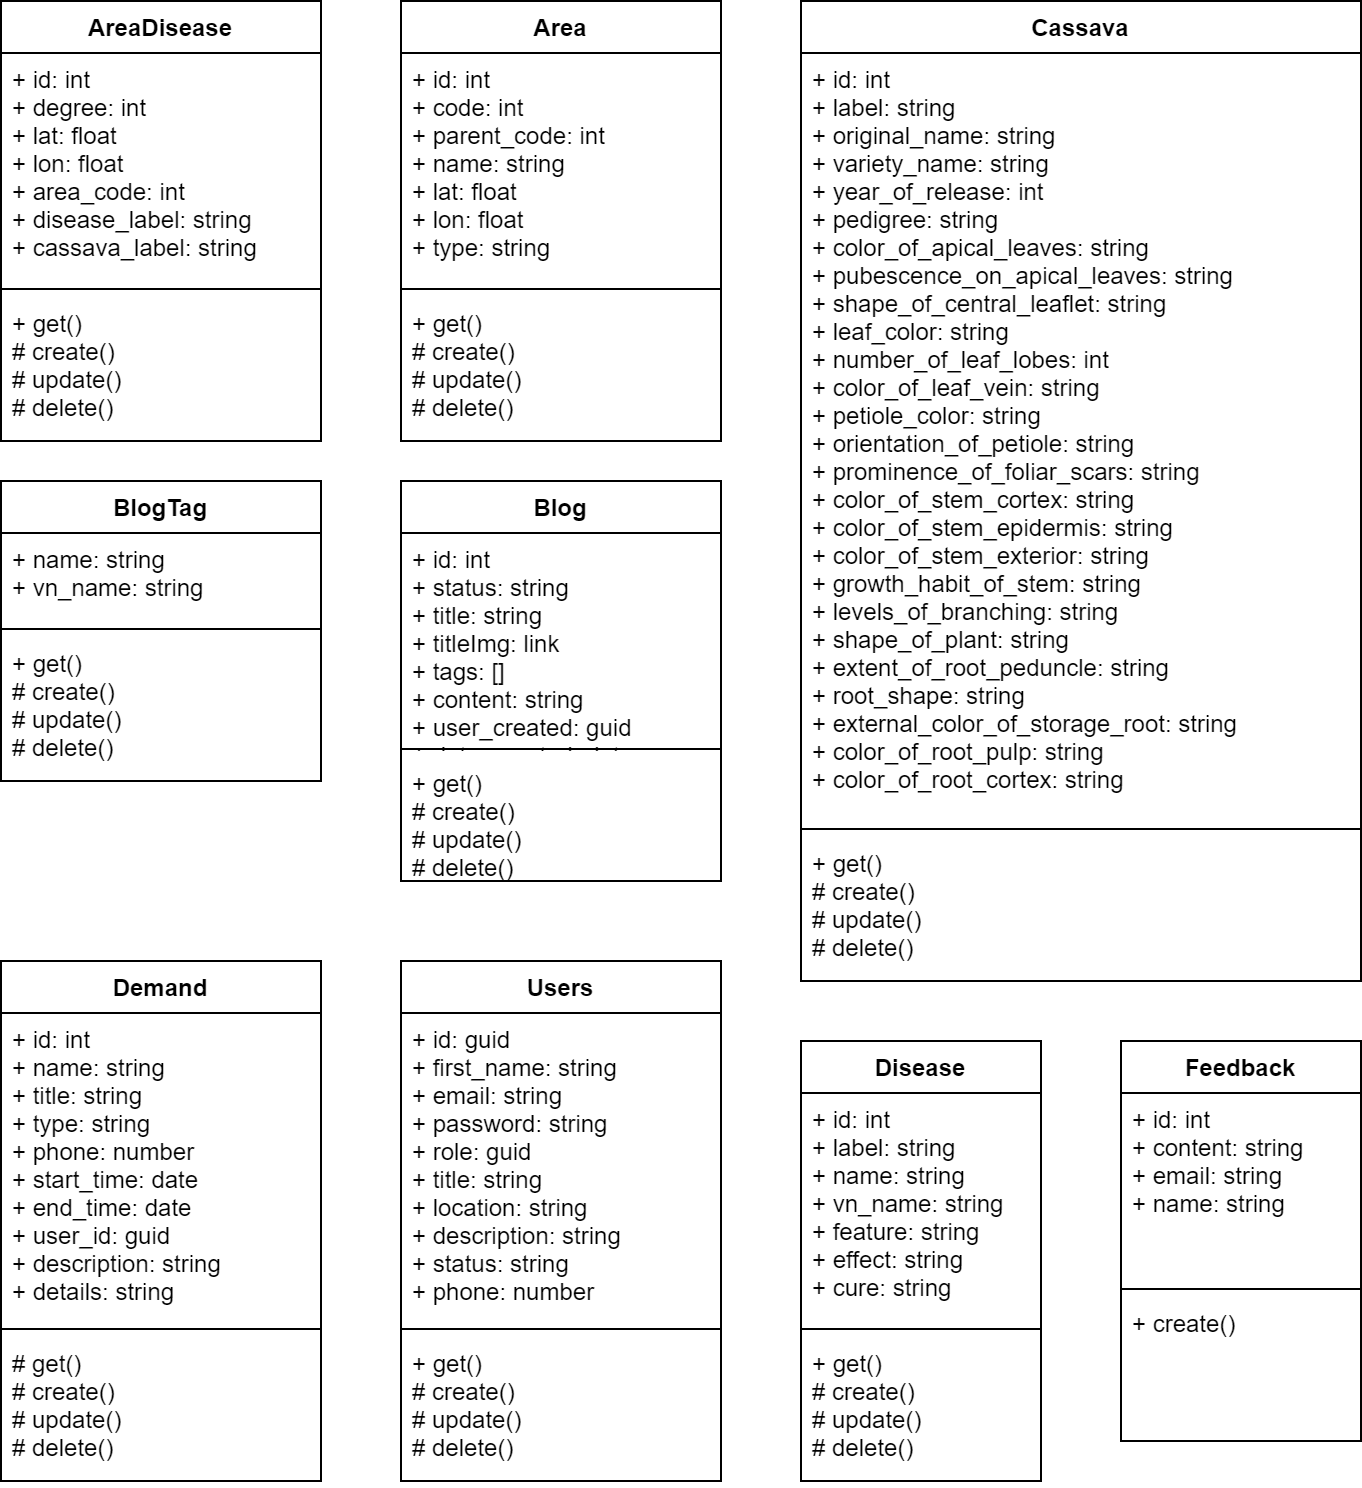
\includegraphics[width=\linewidth]{./img/entities.png}
	\caption{Cơ sở dữ liệu - Các lớp thực thể }
\end{figure}

\subsubsection{Các lớp điều khiển}
Để phục vụ cho việc truy xuất, xử lý dữ liệu, các lớp điều khiển (Controller classes) được thiết kế như sau:
\begin{figure}[H]
	\centering
	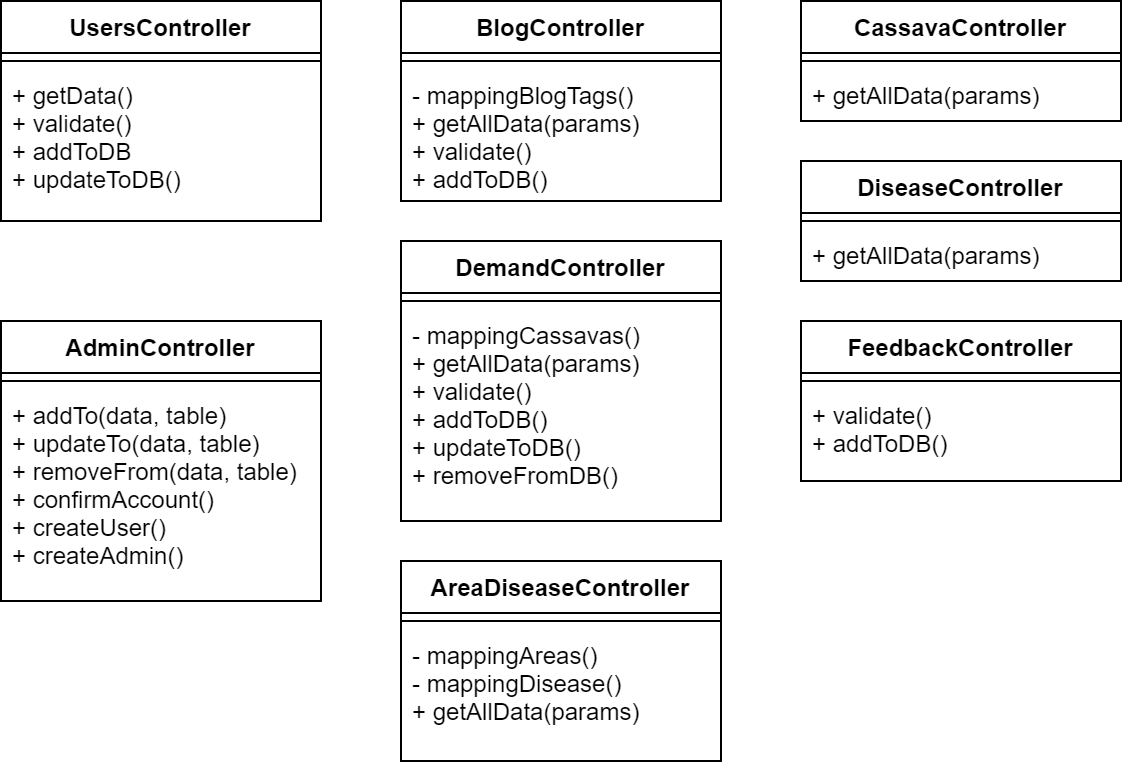
\includegraphics[width=\linewidth]{./img/controller.png}
	\caption{Các lớp điều khiển}
\end{figure}

\subsubsection{Các lớp giao diện}
Các tác nhân sẽ tương tác với hệ thống thông qua các thao tác với các lớp giao diện (Boundary classes):
\begin{figure}[H]
	\centering
	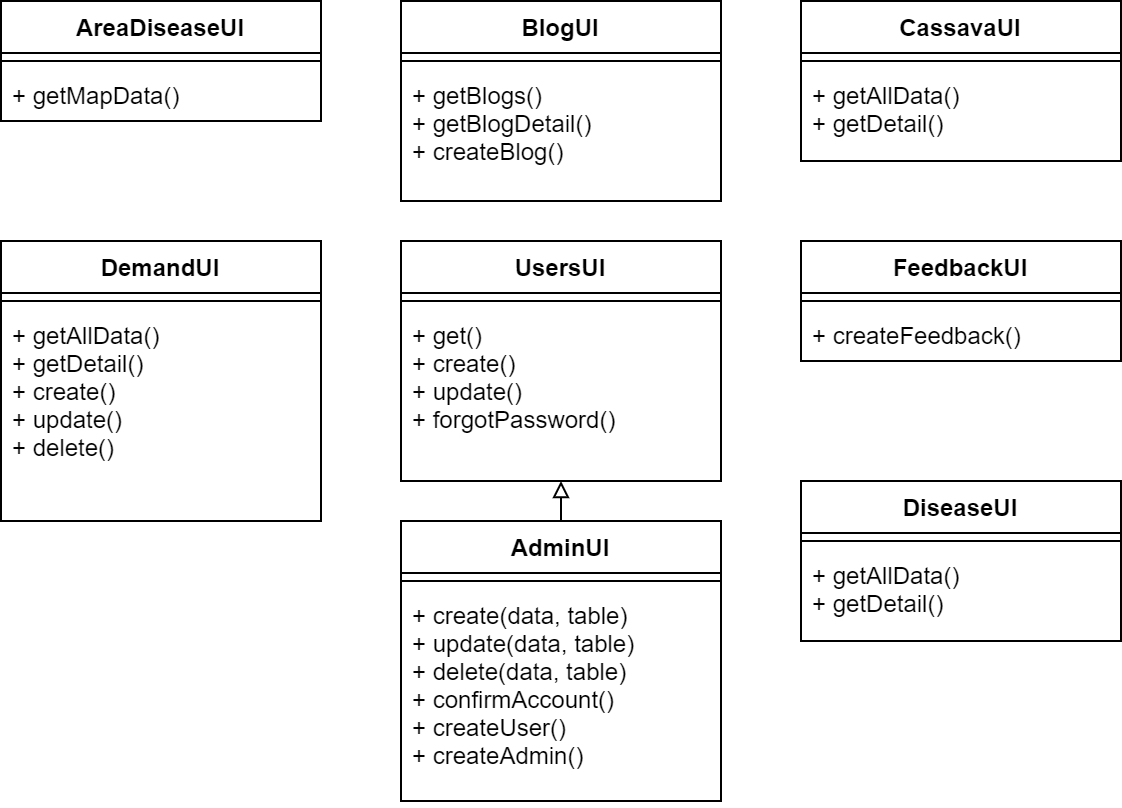
\includegraphics[width=\linewidth]{./img/boundary.png}
	\caption{Các lớp giao diện}
\end{figure}

\subsubsection{Sơ đồ lớp}
Tổng quát sự trao đổi và tương tác của hệ thống được biểu diễn như sau:
\begin{figure}[H]
	\centering
	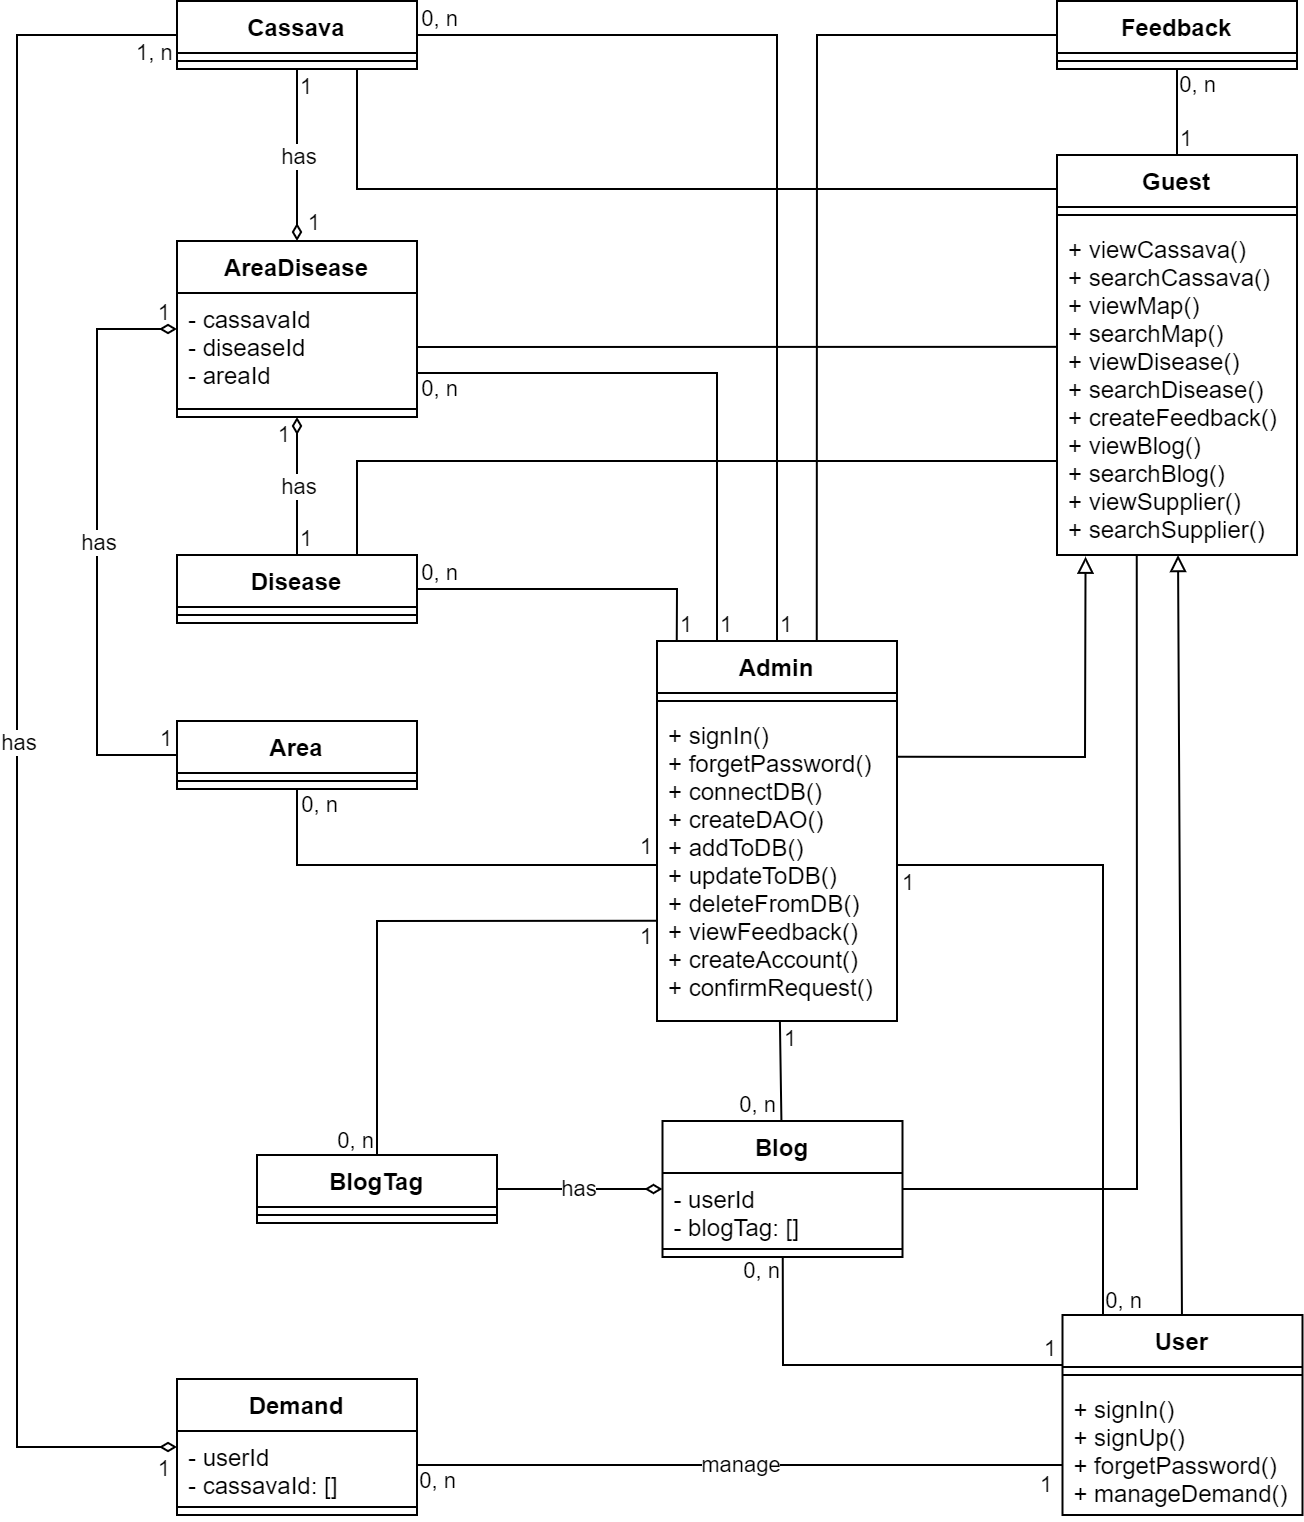
\includegraphics[width=\linewidth]{./img/classes.png}
	\caption{Sơ đồ lớp}
\end{figure}

Sơ đồ lớp (Class diagram) mô tả các quan hệ khác nhau tồn tại giữa các đối tượng trong hệ thống. Được phát triển từ cơ sở dữ liệu với các trường dữ liệu tương tự với trong các lớp thực thể, ngoài ra sẽ có thêm các hàm khác phụ trợ cho việc trao đổi dữ liệu, tương tác với nhau giữa các đối tượng. Các đường liên kết giữa các đối tượng biểu thị mối quan hệ liên kết, kế thừa, thu nạp và mối quan hệ một - một, một - nhiều, nhiều nhiều - nhiều, mối quan hệ bắt buộc và không bắt buộc.

Các tương tác giữa các đối tượng sẽ được miêu tả cụ thể trong phần biểu đồ tuần tự dưới đây.

\subsection{Biểu đồ tuần tự}

\subsubsection{Đăng ký}
\begin{figure}[H]
	\centering
	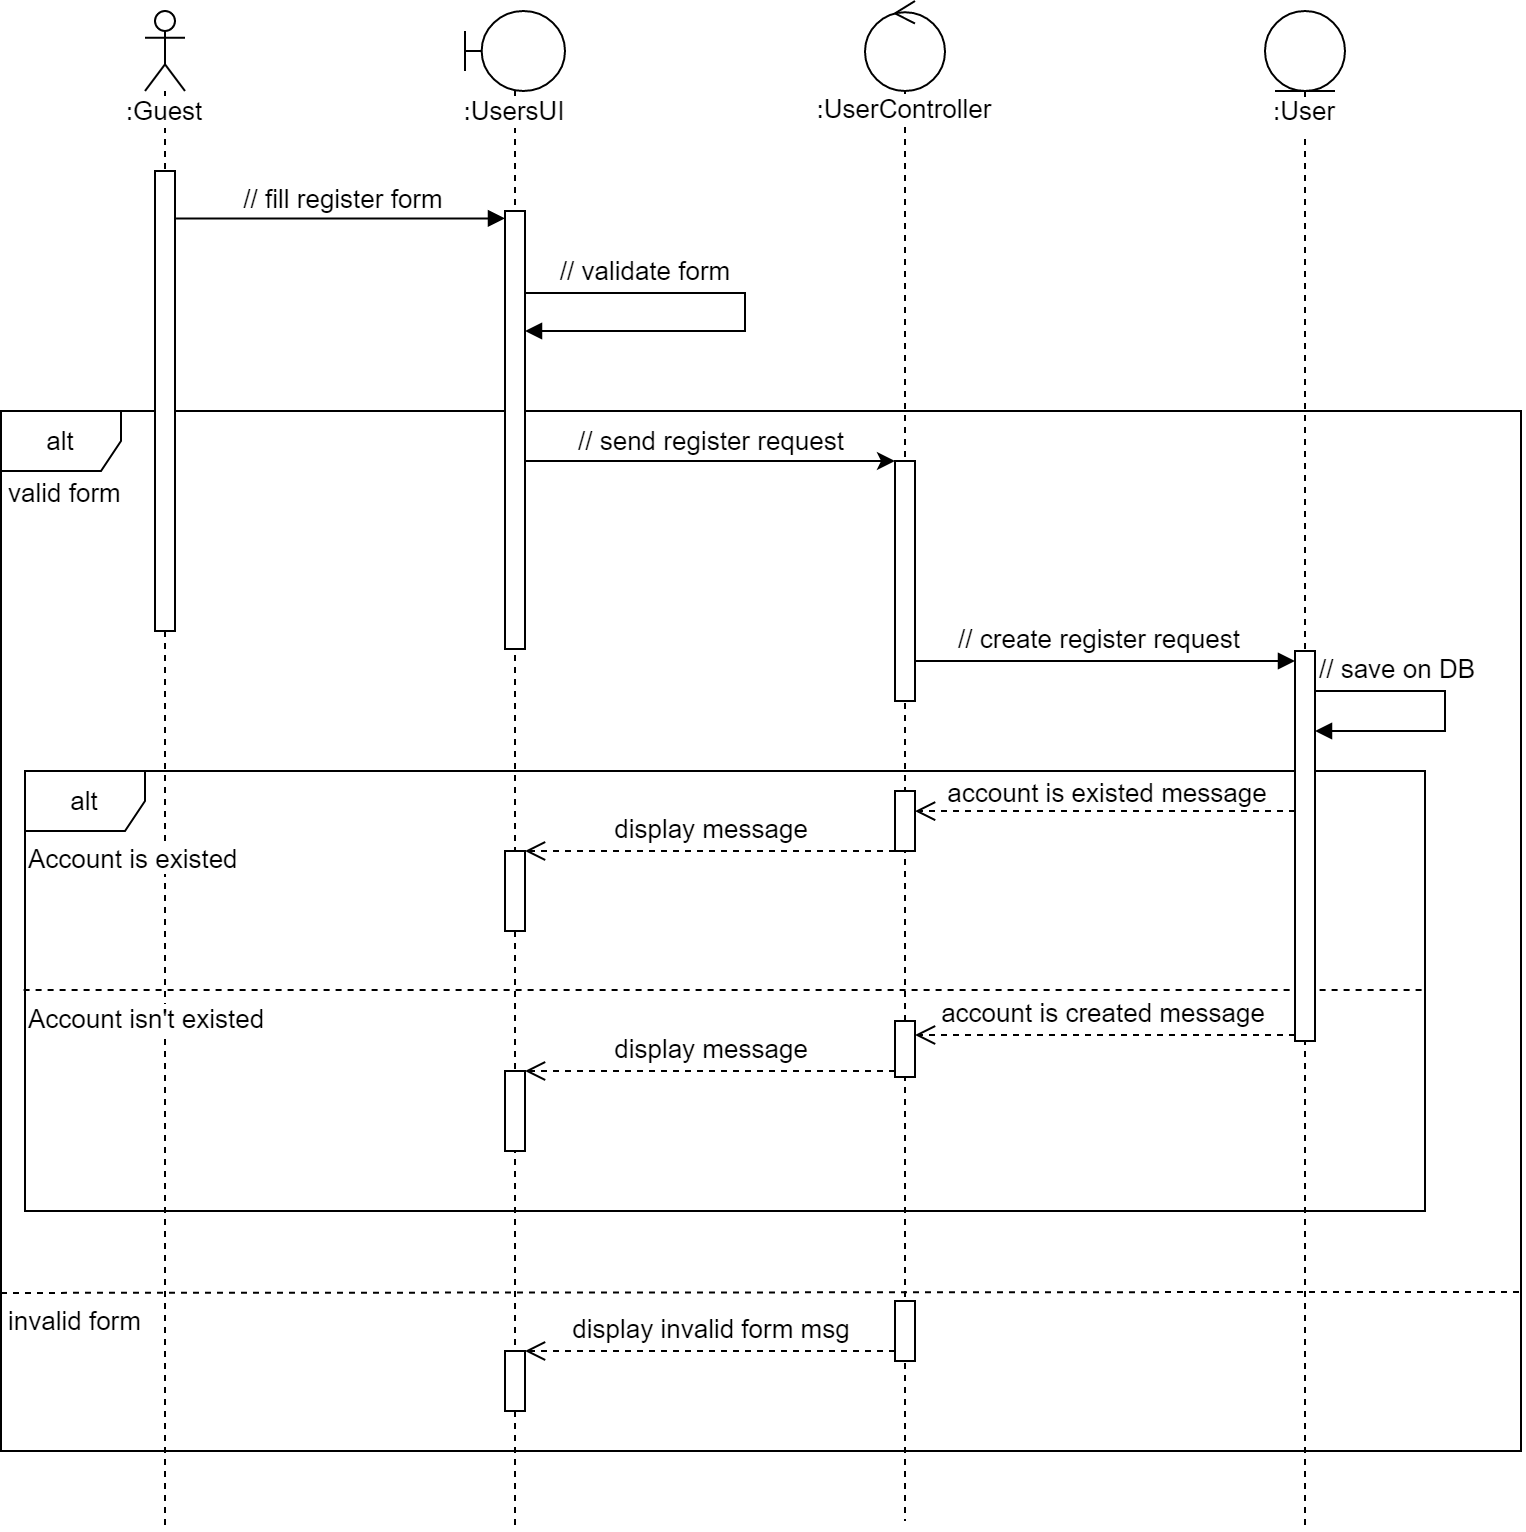
\includegraphics[width=\linewidth]{./img/uc1.png}
	\caption{Biểu đồ tuần tự - Ca sử dụng Đăng ký}
\end{figure}

\subsubsection{Đăng nhập}
\begin{figure}[H]
	\centering
	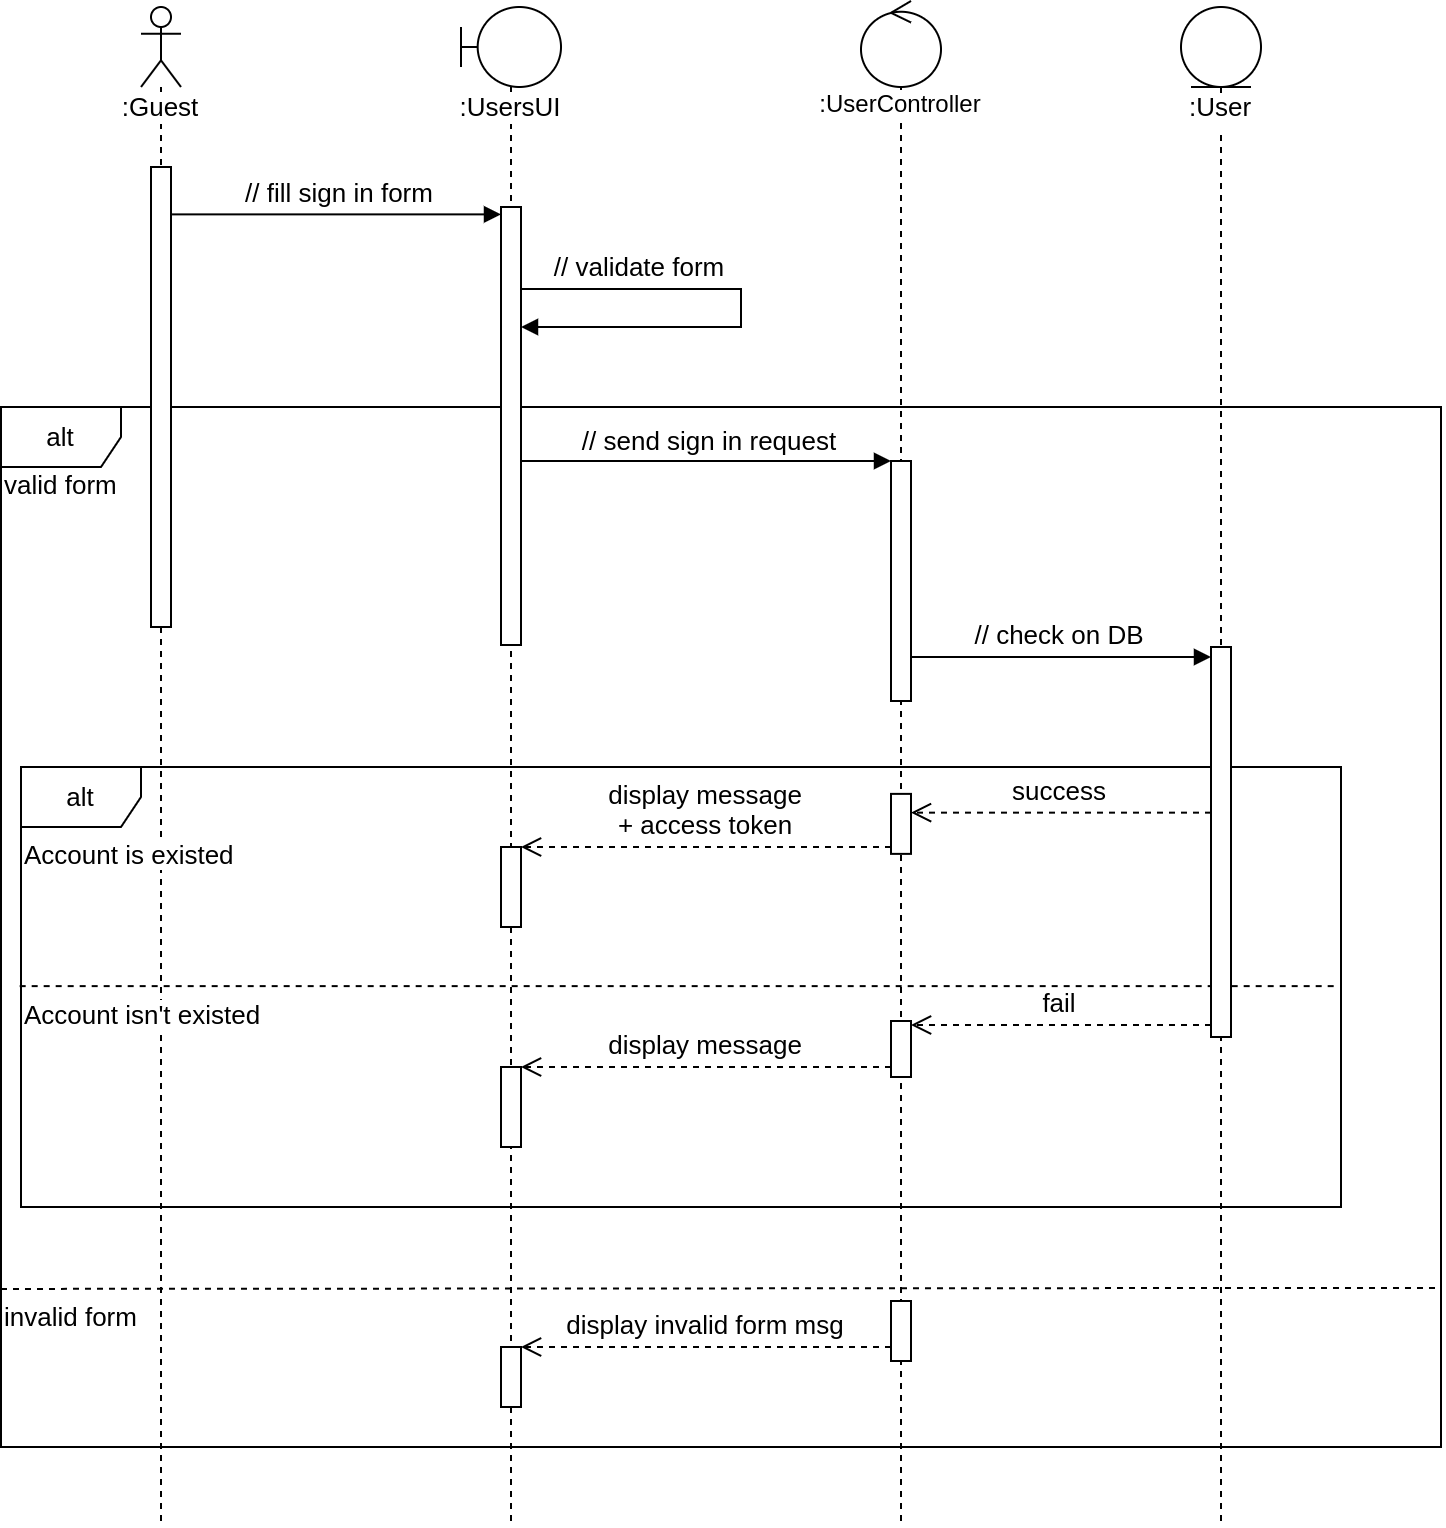
\includegraphics[width=\linewidth]{./img/uc2.png}
	\caption{Biểu đồ tuần tự - Ca sử dụng Đăng nhập}
\end{figure}

\subsubsection{Quên mật khẩu}
\begin{figure}[H]
	\centering
	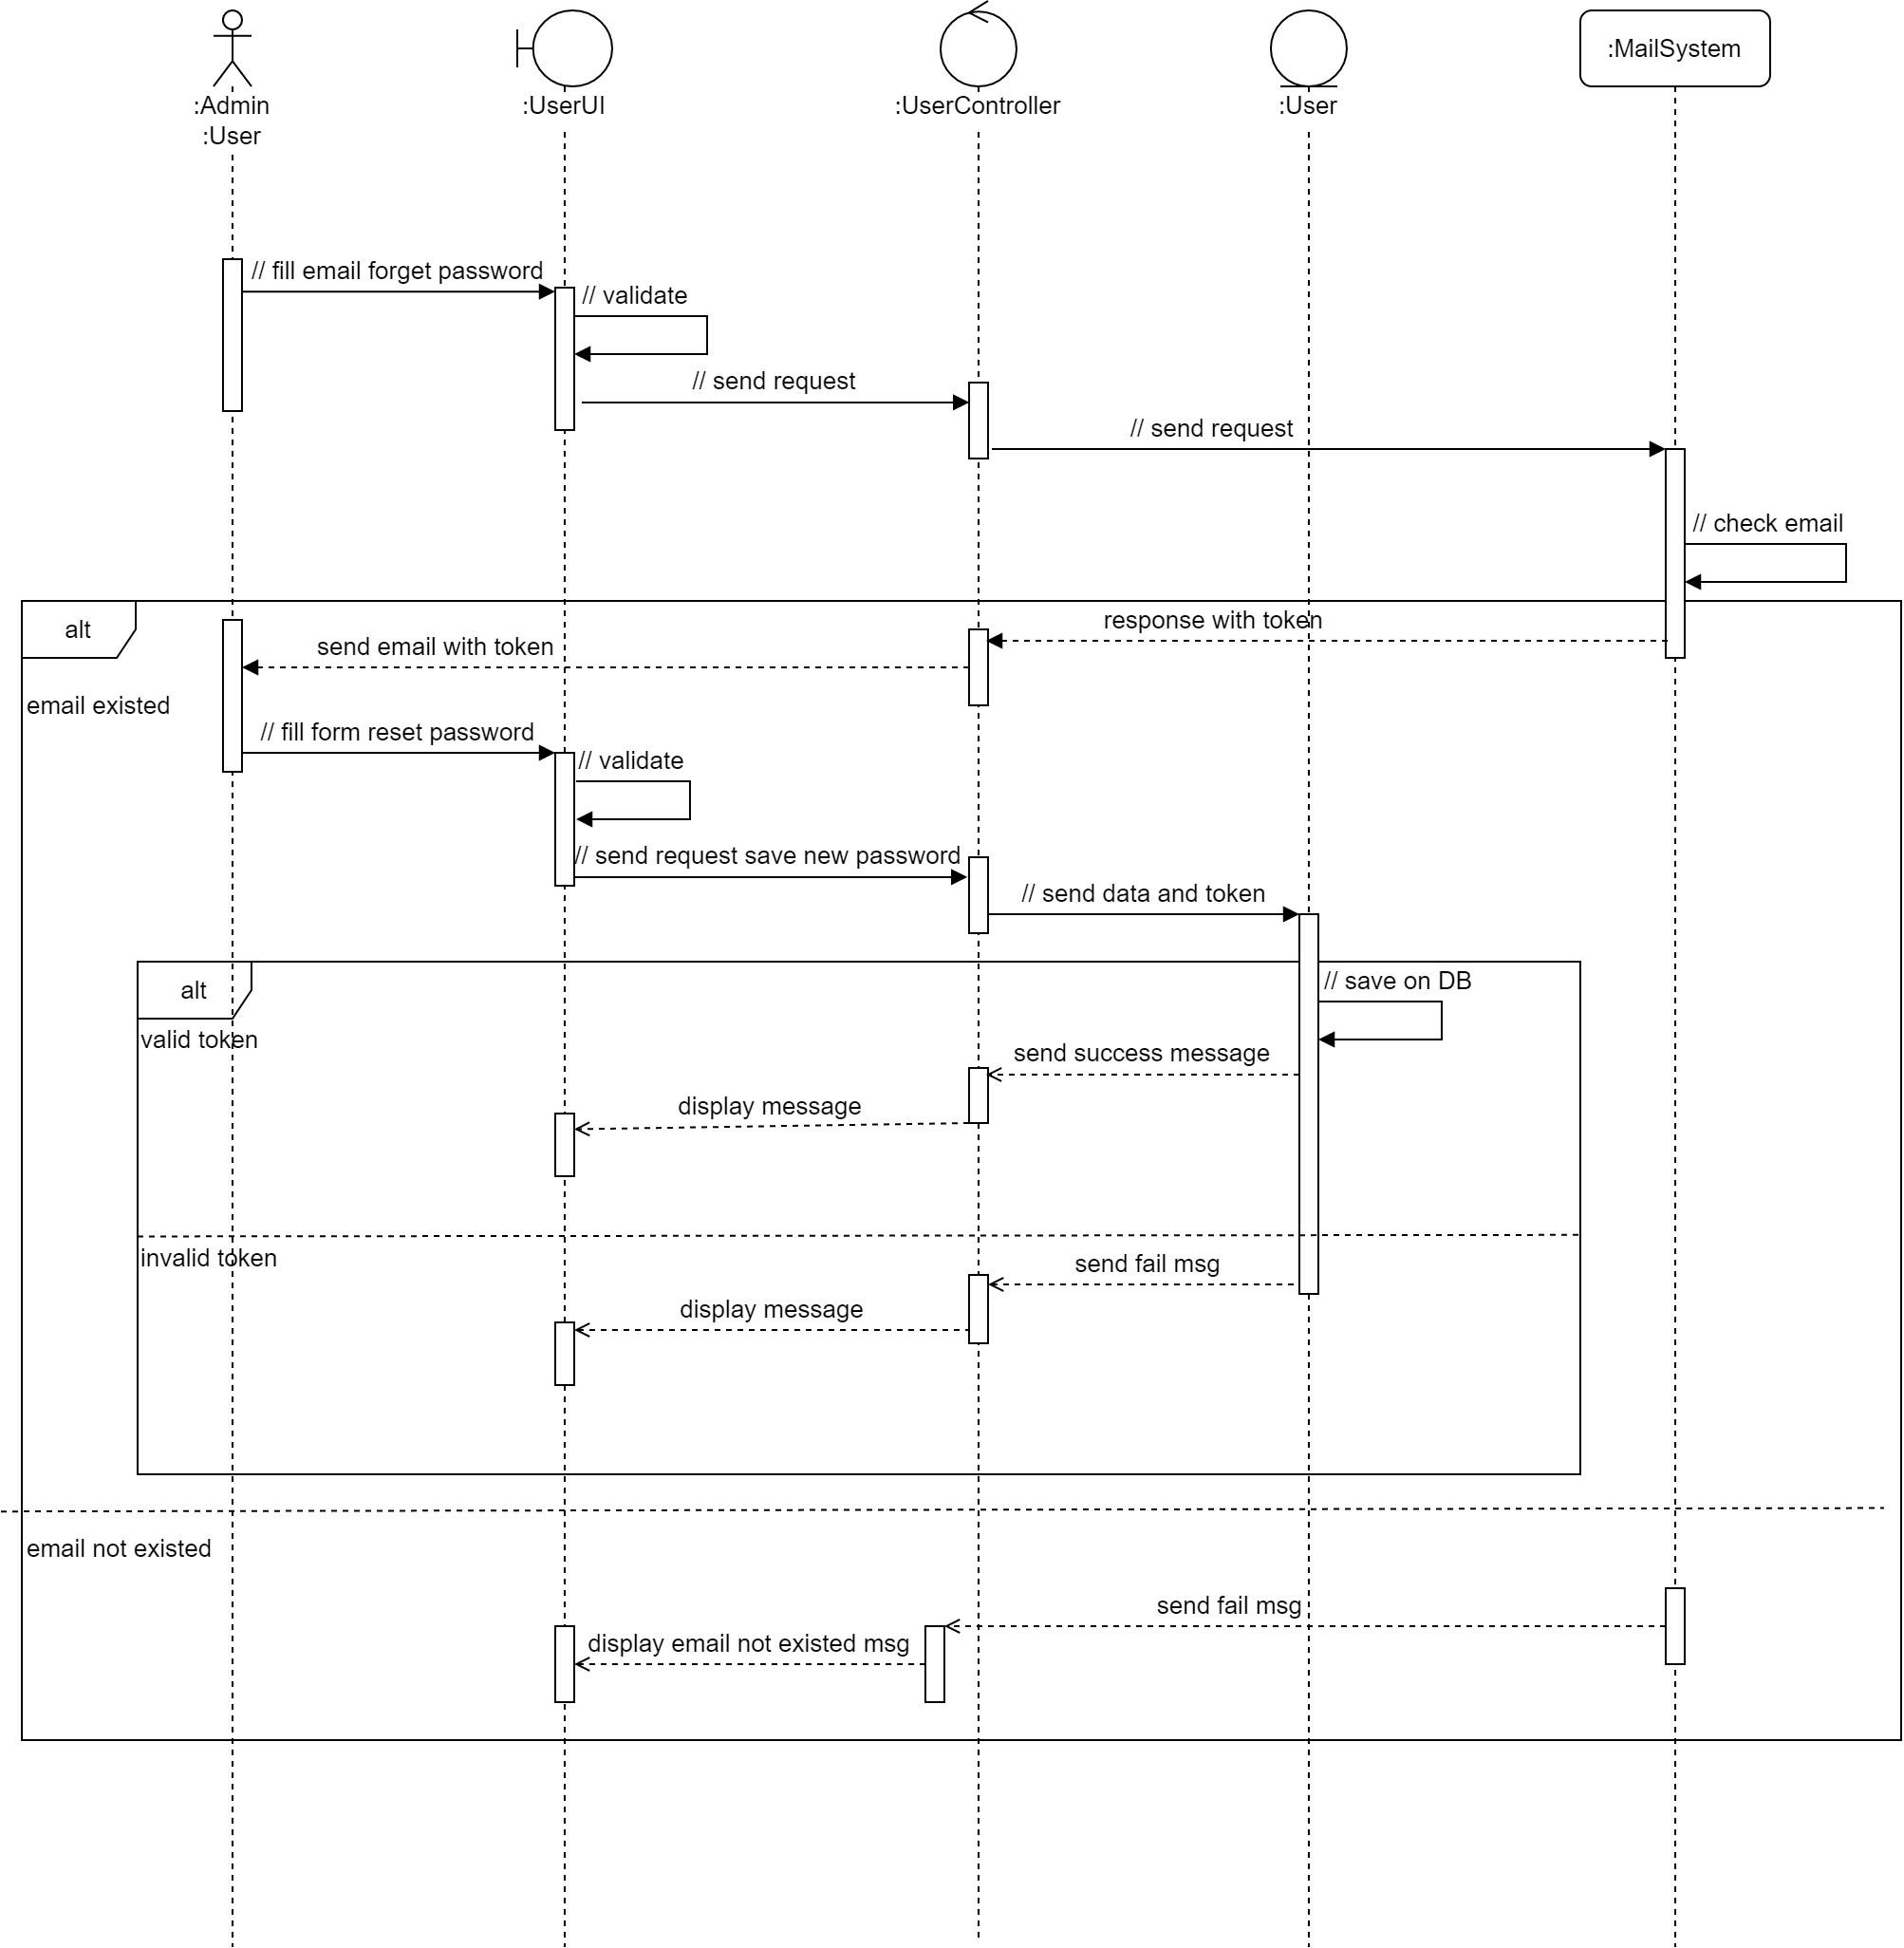
\includegraphics[width=\linewidth]{./img/uc3.png}
	\caption{Biểu đồ tuần tự - Ca sử dụng Quên mật khẩu}
\end{figure}

Trong ca sử dụng Quên mật khẩu hệ thống có sử dụng SMTP của Gmail để gửi thư điện tử kèm đường dẫn giúp người dùng đổi mật khẩu.

SMTP \cite{smtp} (tiếng Anh: Simple Mail Transfer Protocol - giao thức truyền tải thư tín đơn giản) là một chuẩn truyền tải thư điện tử qua mạng Internet. SMTP được định nghĩa trong bản RFC 821 (STD 10) và được chỉnh lý bằng bản RFC 1123 (STD 3), chương 5. Địa chỉ máy chủ SMTP của Gmail là smtp.gmail.com.

Khi người dùng gửi yêu cầm quên mật khẩu kèm email đã đăng ký, hệ thống sẽ thông qua SMTP gửi lại đường dẫn có chứa token đến trang đổi mật khẩu cho người dùng. Token có hạn sử dụng trong vòng 24 giờ kể từ khi hệ thống gửi thư điện tử. Nếu token còn hợp lệ thì khi cập nhật mới khẩu mới sẽ thành công. Nếu không thì mật khẩu vẫn giữ nguyên, không được thay đổi. Người dùng cần phải gửi yêu cầu quên mật khẩu mới nếu muốn thay đổi mật khẩu.

\subsubsection{Sửa thông tin tài khoản}
\begin{figure}[H]
	\centering
	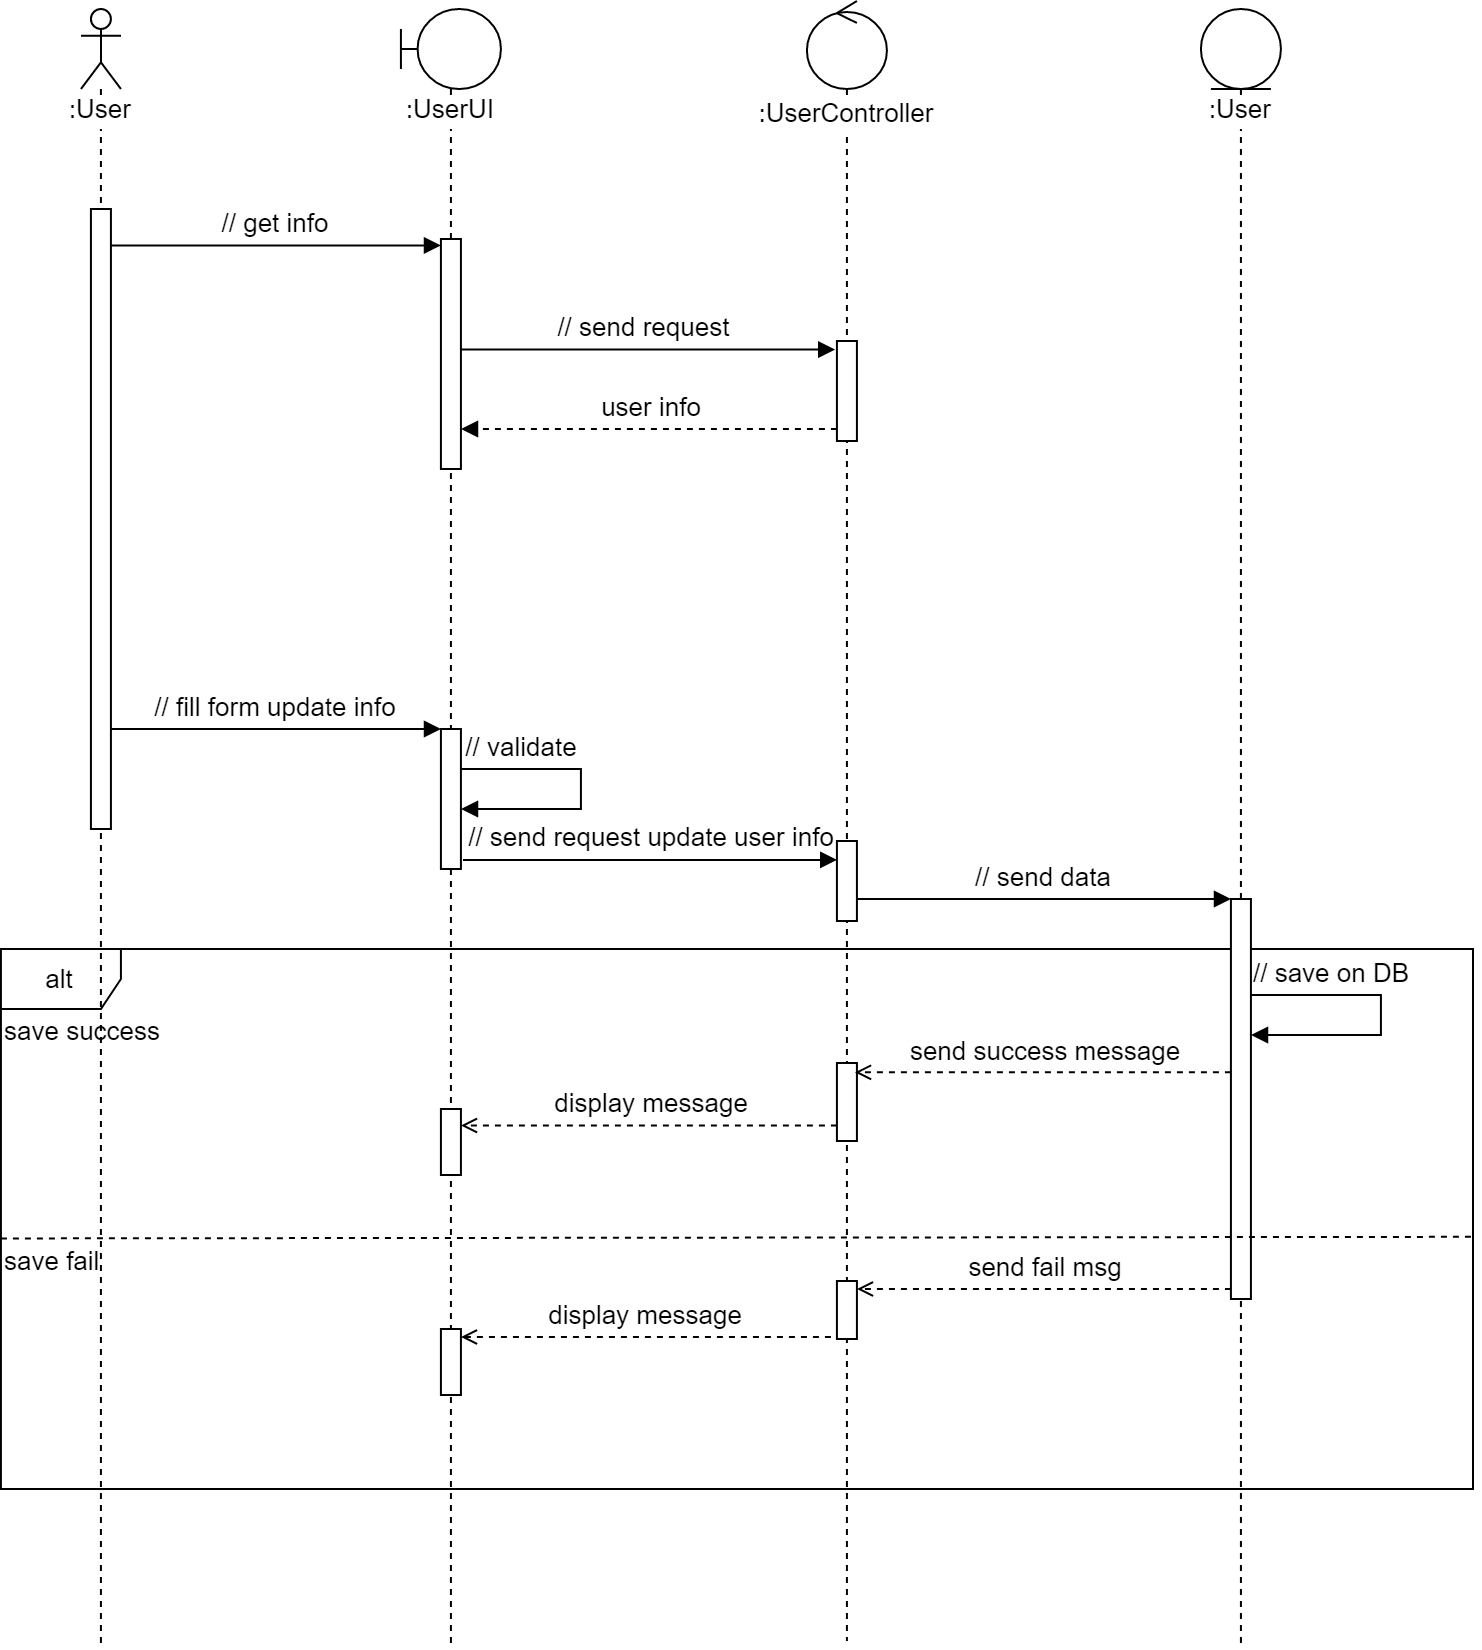
\includegraphics[width=\linewidth]{./img/uc4.png}
	\caption{Biểu đồ tuần tự - Ca sử dụng Sửa thông tin tài khoản}
\end{figure}

\subsubsection{Đăng xuât}
\begin{figure}[H]
	\centering
	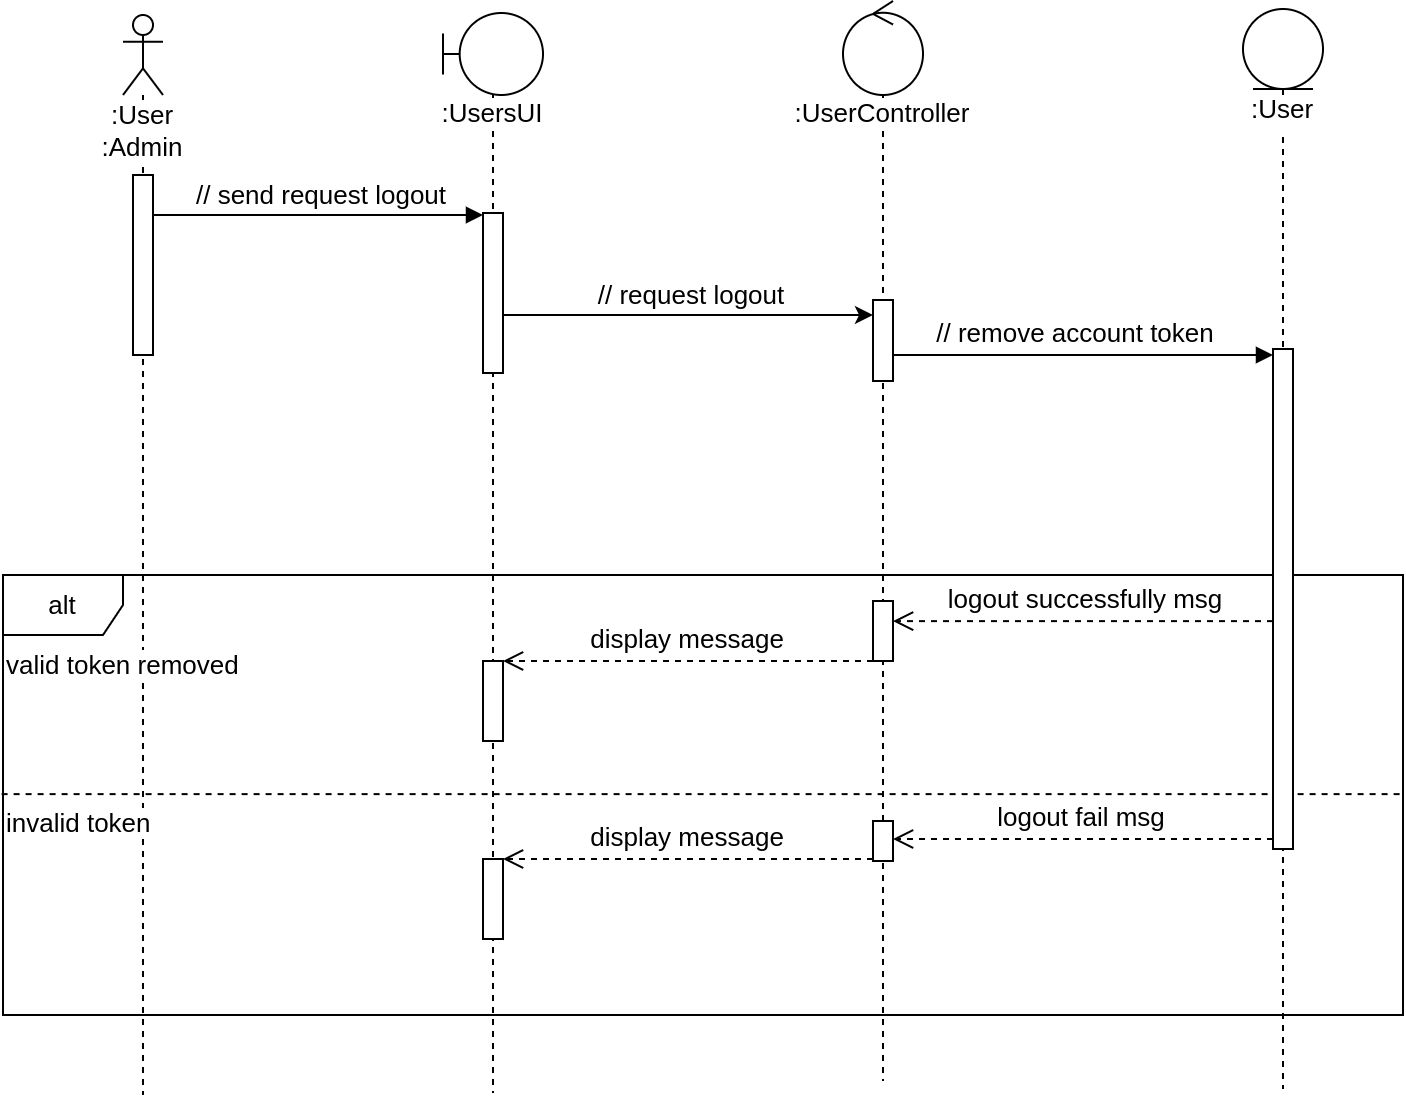
\includegraphics[width=\linewidth]{./img/uc5.png}
	\caption{Biểu đồ tuần tự - Ca sử dụng Đăng xuât}
\end{figure}

\subsubsection{Các ca sử dụng xem và tìm kiếm dữ liệu}
\begin{figure}[H]
	\centering
	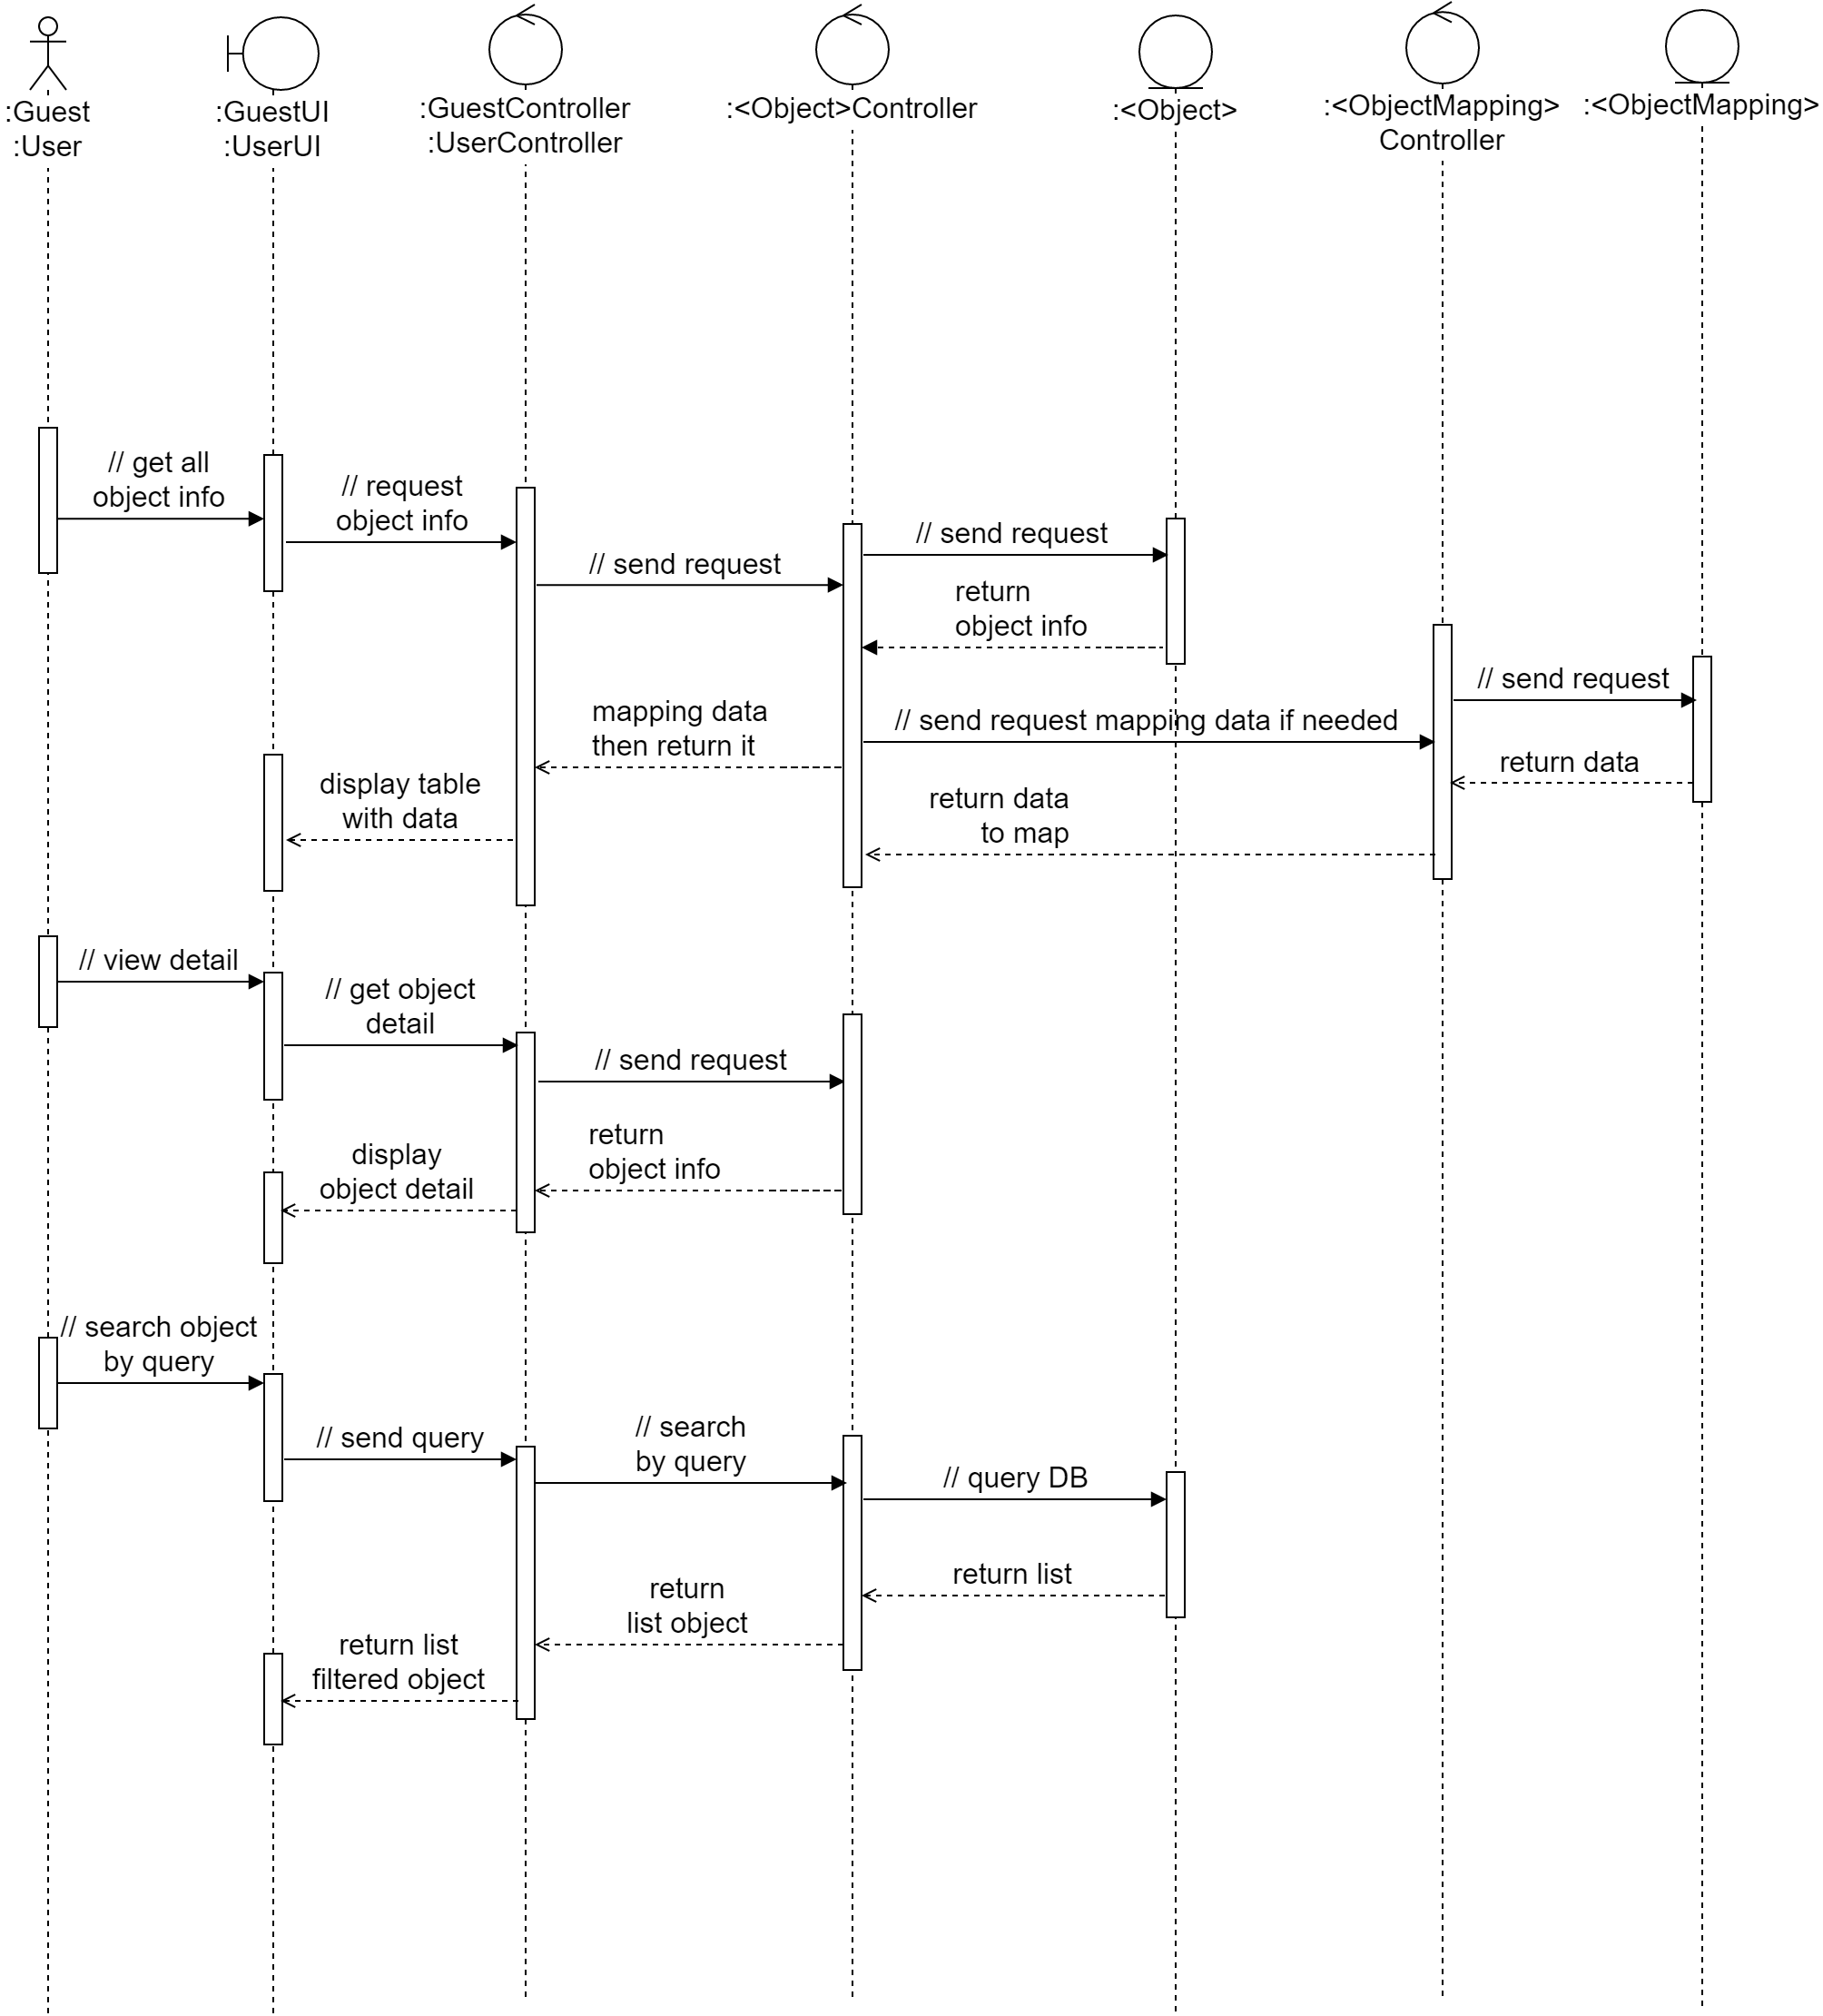
\includegraphics[width=\linewidth]{./img/uc6-11.png}
	\caption{Biểu đồ tuần tự - Các ca sử dụng xem và tìm kiếm dữ liệu}
\end{figure}

Các ca sử dụng xem và tìm kiếm dữ liệu có thể khá tương đồng nhau trong luồng hoạt động. Có một số bảng dữ liệu không cần liên kết với các bảng dữ liệu khác để hiển thị đầy đủ thông tin, chúng có thể đứng độc lập, như là: dữ liệu về sắn, bệnh về sắn,... Tuy nhiên cũng có những bảng dữ liệu cần liên kết với một hay nhiều bảng dữ liệu khác để hiển thị được đầy đủ, chẳng hạn: dữ liệu về bản đồ sắn, dữ liệu về thương mại sắn,...

Cụ thể bảng dữ liệu về bản đồ sắn biểu thị thông tin về dịch bệnh sắn ở Tây Ninh trên bản đồ cần liên kết với bảng dữ liệu sắn thông qua nhãn sắn, bệnh về sắn thông qua nhãn bệnh cũng như tọa độ địa lý các khu vực ở Tây Ninh thông qua mã khu vực, từ đó hiển thị được đúng và đủ dữ liệu.

Để phục vụ cho việc vẽ bản đồ, hệ thống sử dụng Leaflet \cite{leafletjs} (thư viện viết bằng javascript với mã nguồn mở có khả năng tương thích trên điện thoại di động và cho phép người dùng tương tác trên bản vẽ).

\subsubsection{Chẩn đoán bệnh trên cây sắn}
\begin{figure}[H]
	\centering
	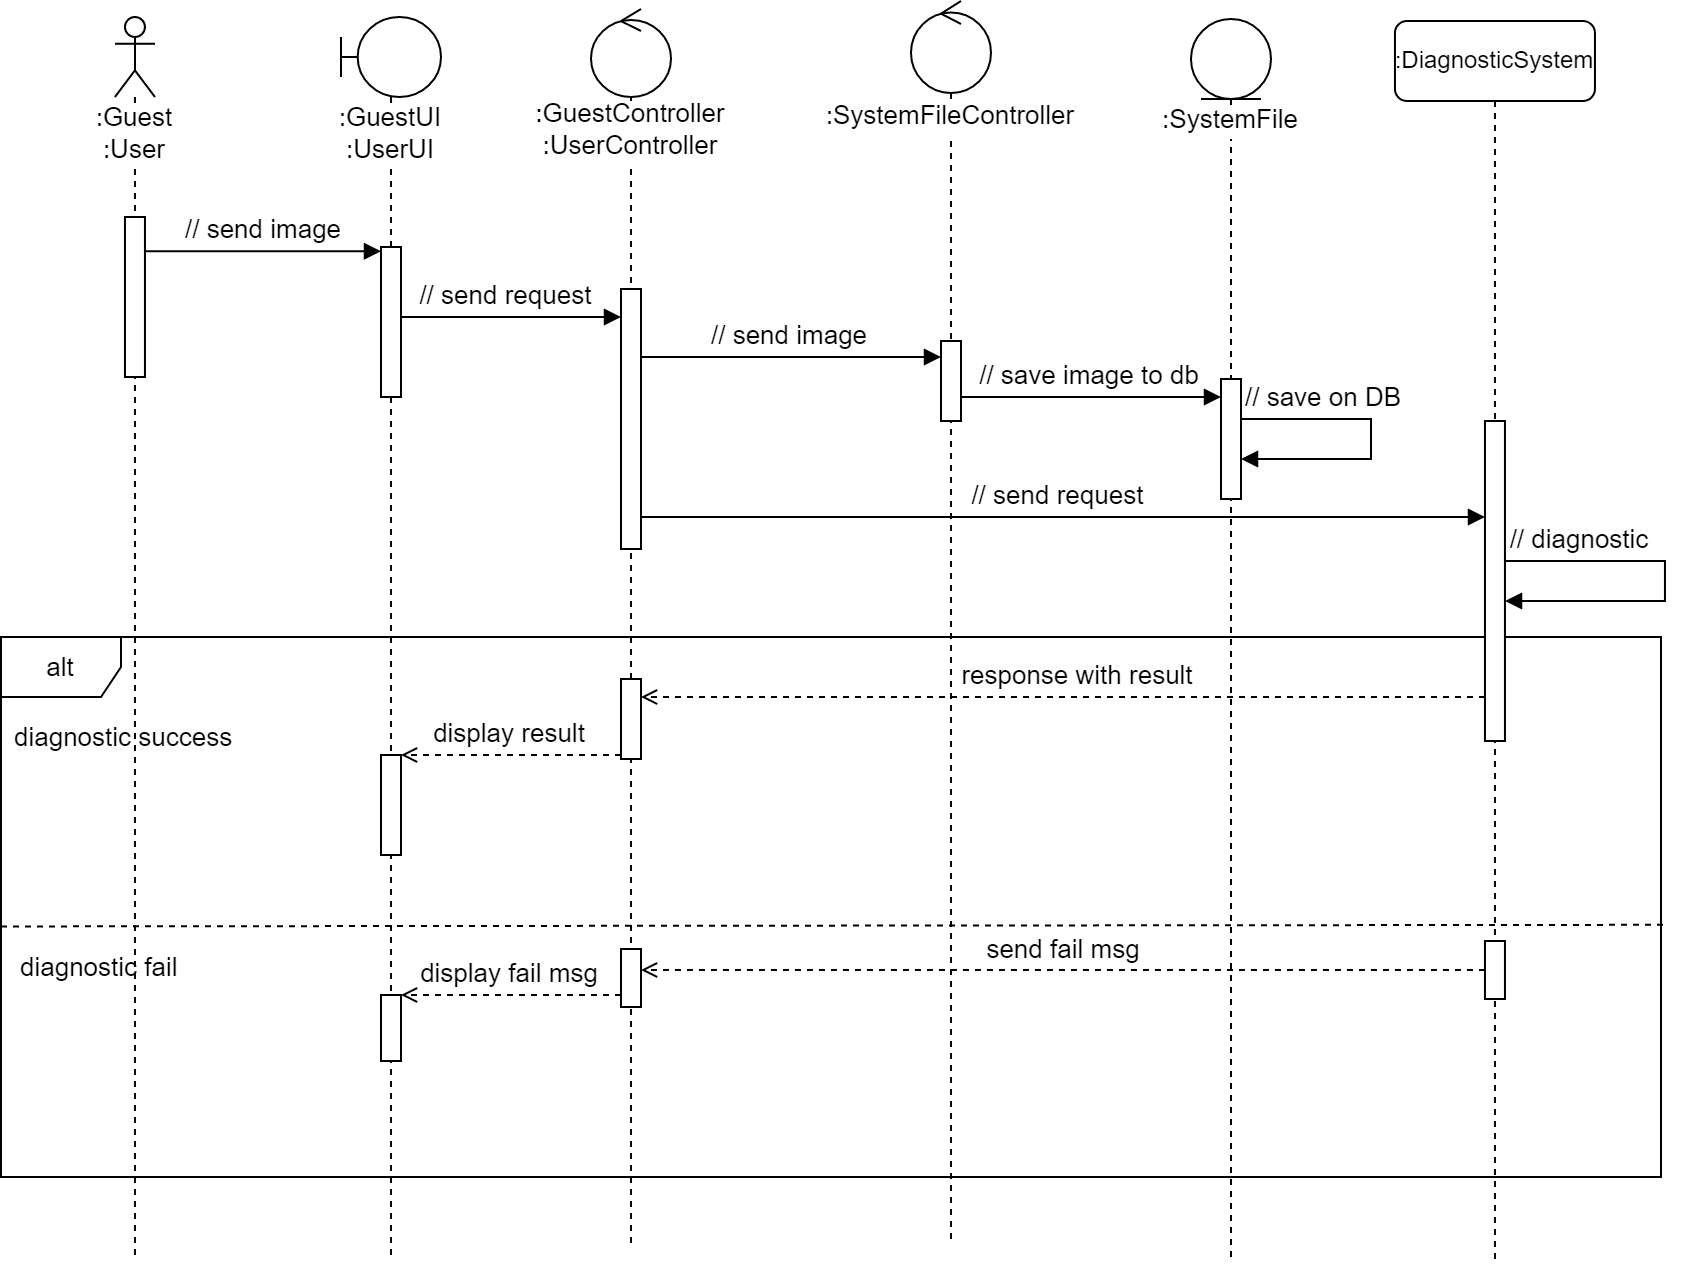
\includegraphics[width=\linewidth]{./img/uc12.png}
	\caption{Biểu đồ tuần tự - Ca sử dụng Chẩn đoán bệnh trên cây sắn}
\end{figure}

\subsubsection{Tạo nhận xét}
\begin{figure}[H]
	\centering
	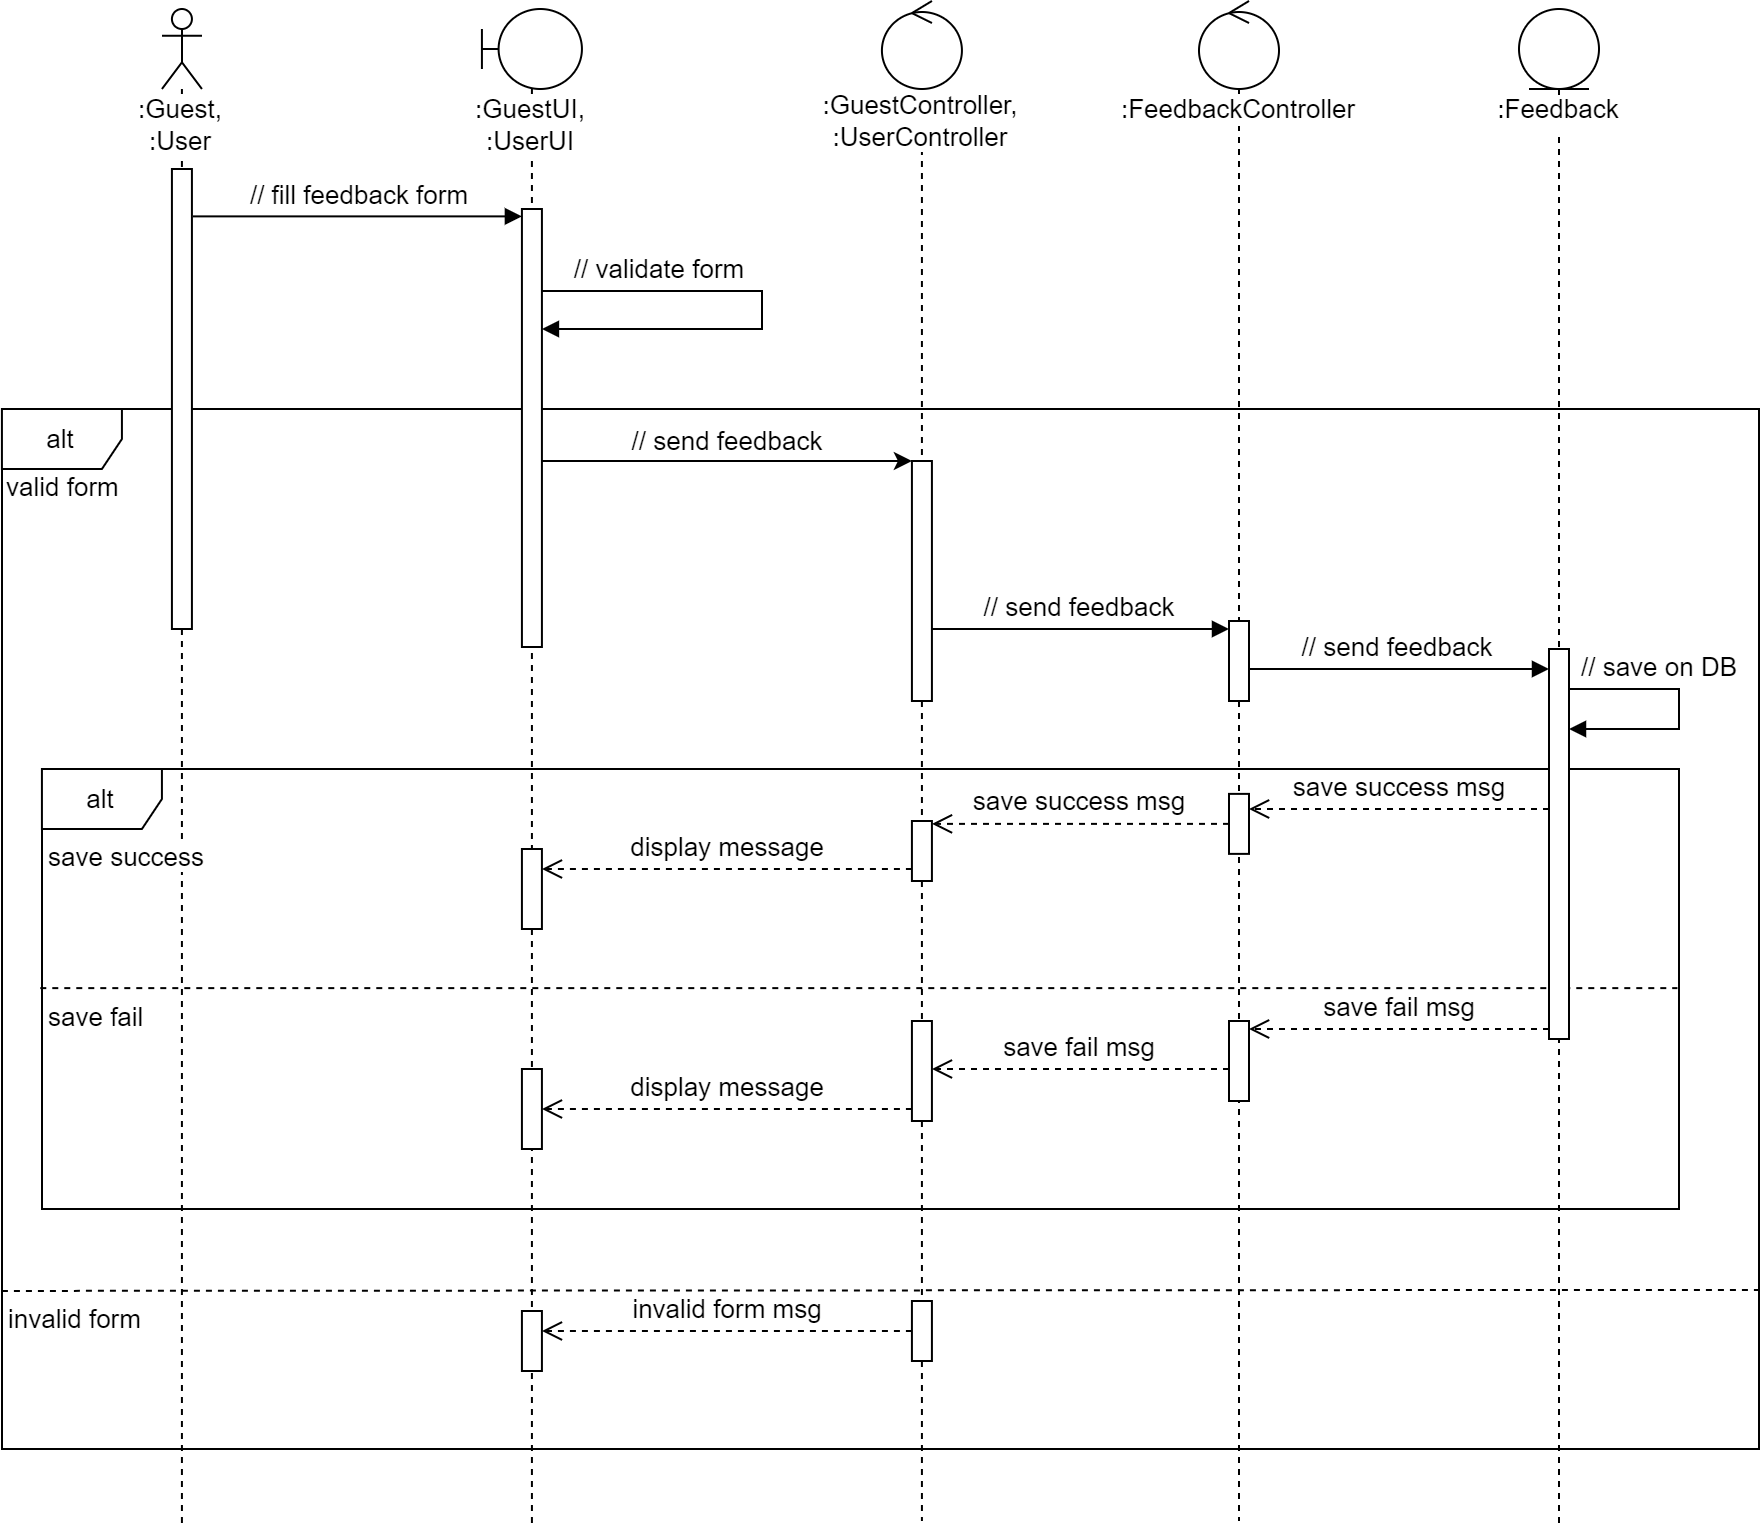
\includegraphics[width=\linewidth]{./img/uc13.png}
	\caption{Biểu đồ tuần tự - Ca sử dụng Tạo nhận xét}
\end{figure}

\subsubsection{Quản lý đề xuất trên sàn thương mại sắn}
\begin{figure}[H]
	\centering
	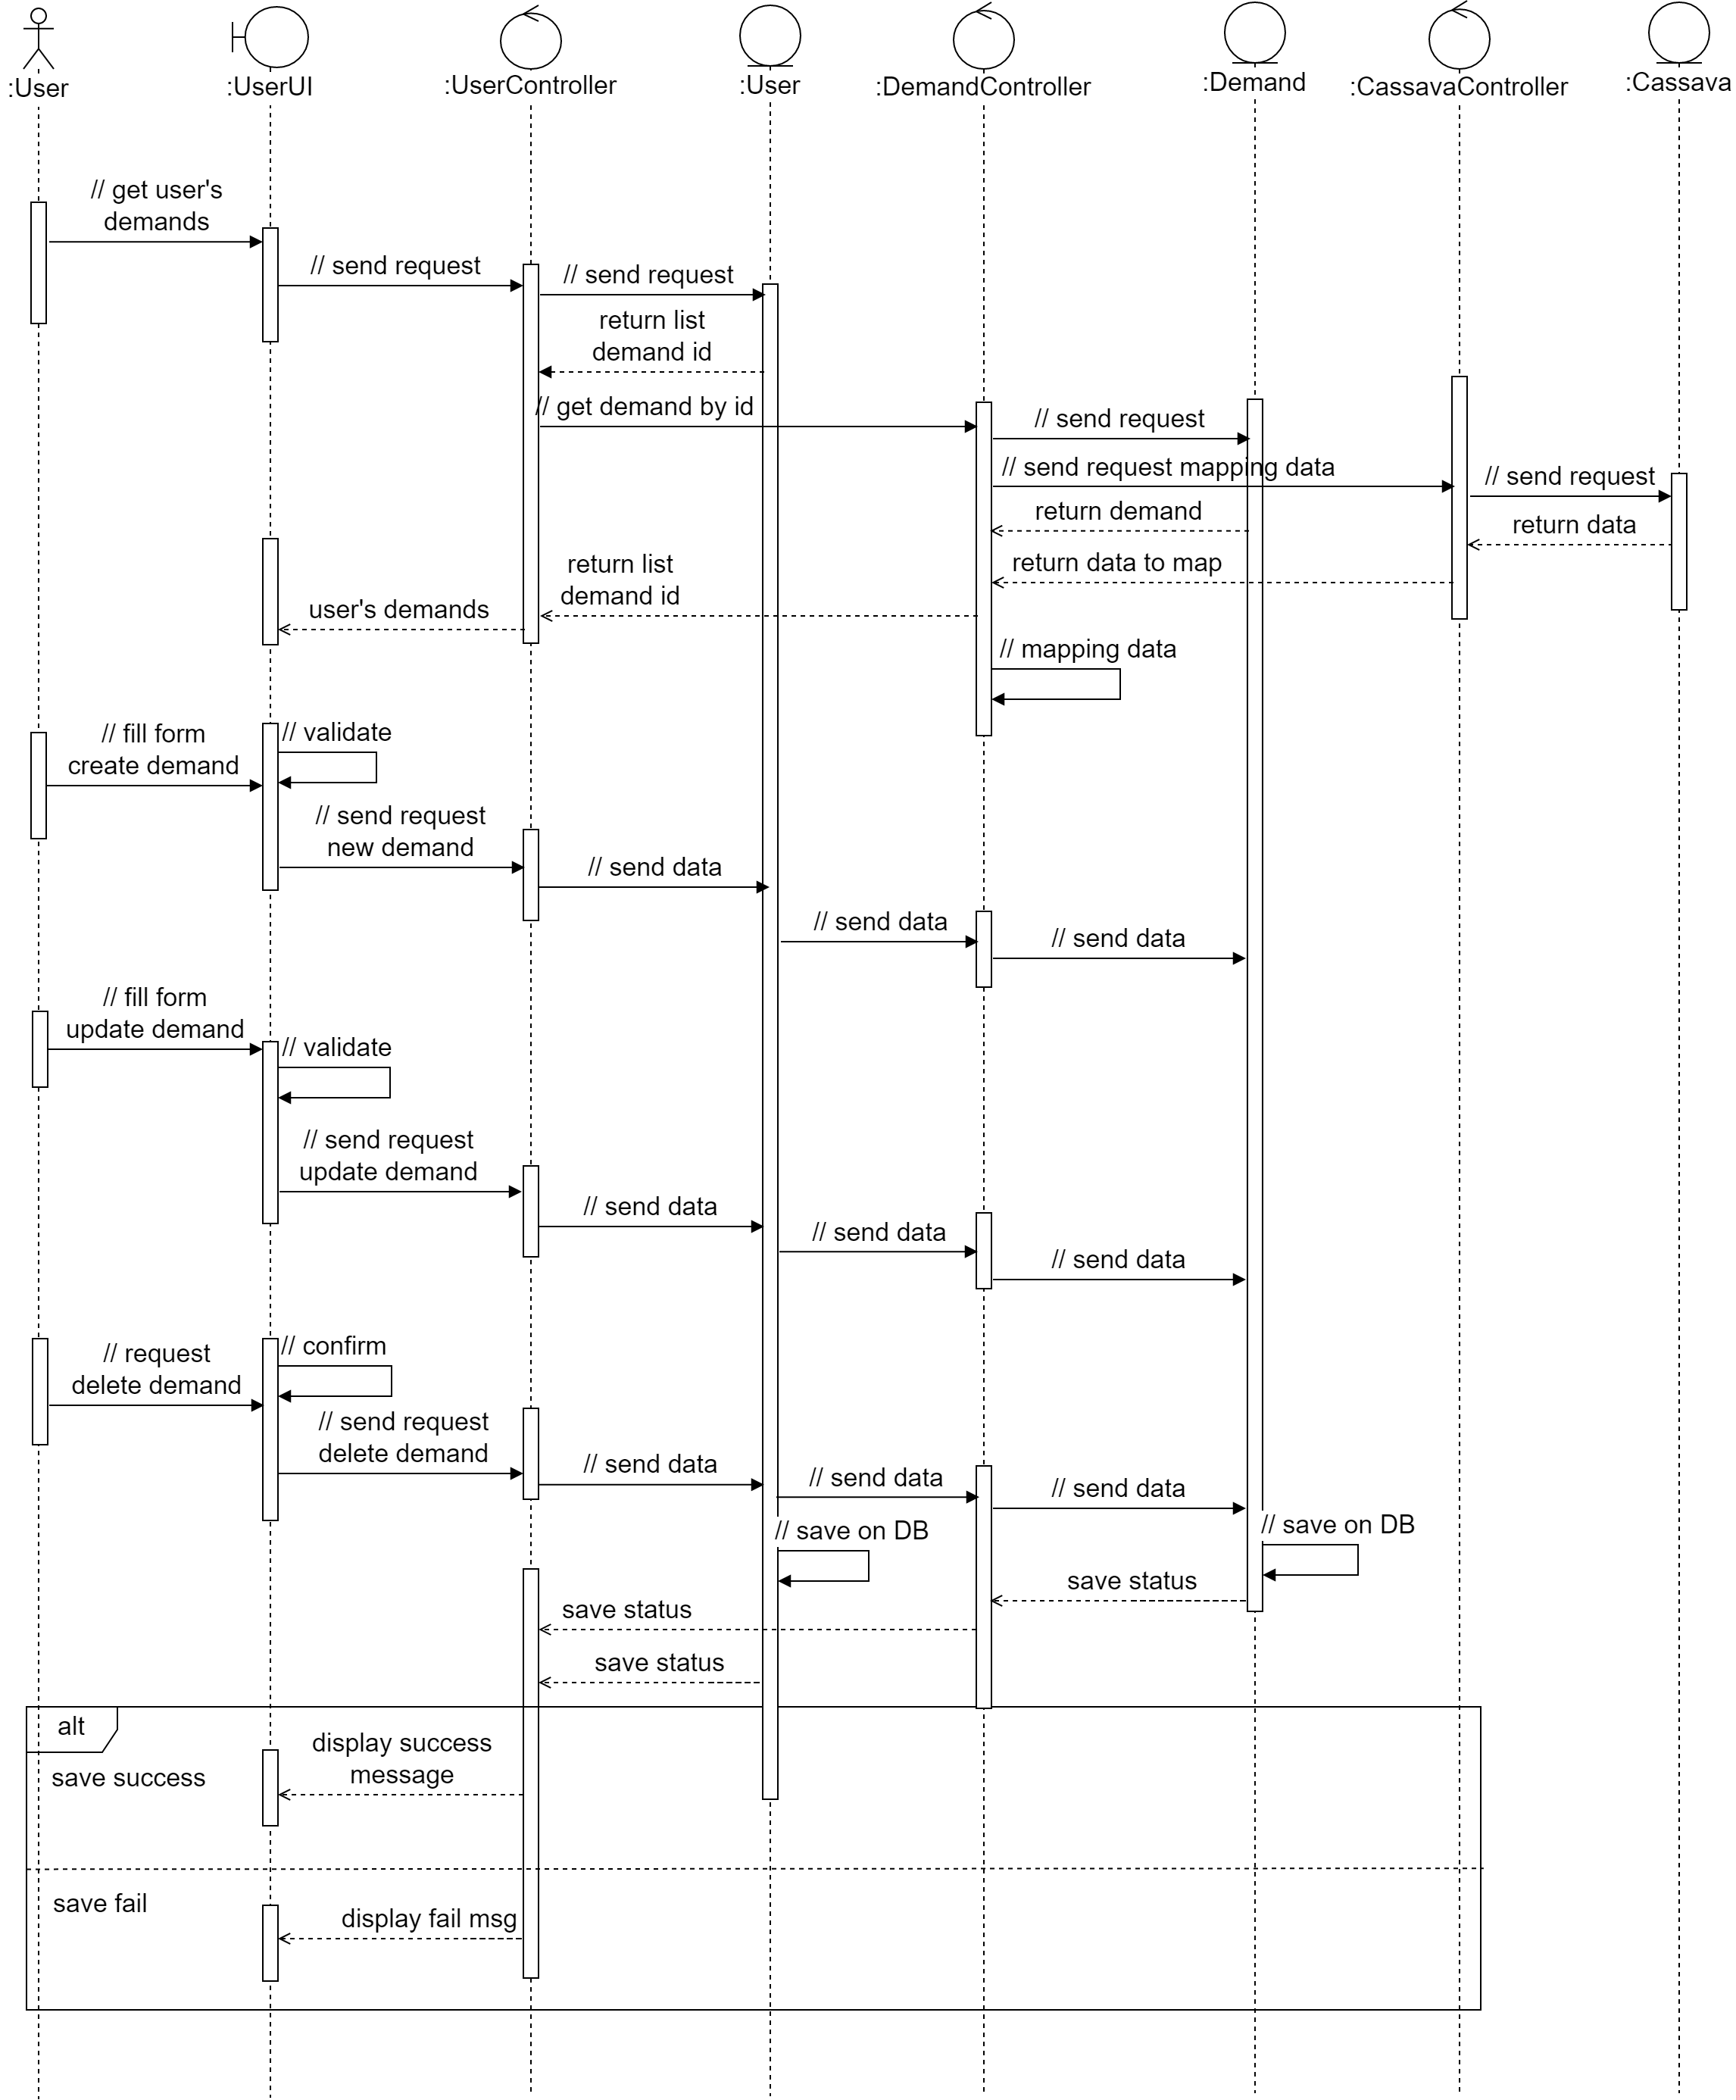
\includegraphics[width=\linewidth]{./img/uc14.png}
	\caption{Biểu đồ tuần tự - Ca sử dụng Quản lý đề xuất trên sàn thương mại sắn}
\end{figure}

\subsubsection{Tạo bài viết trên diễn đàn}

\begin{figure}[H]
	\centering
	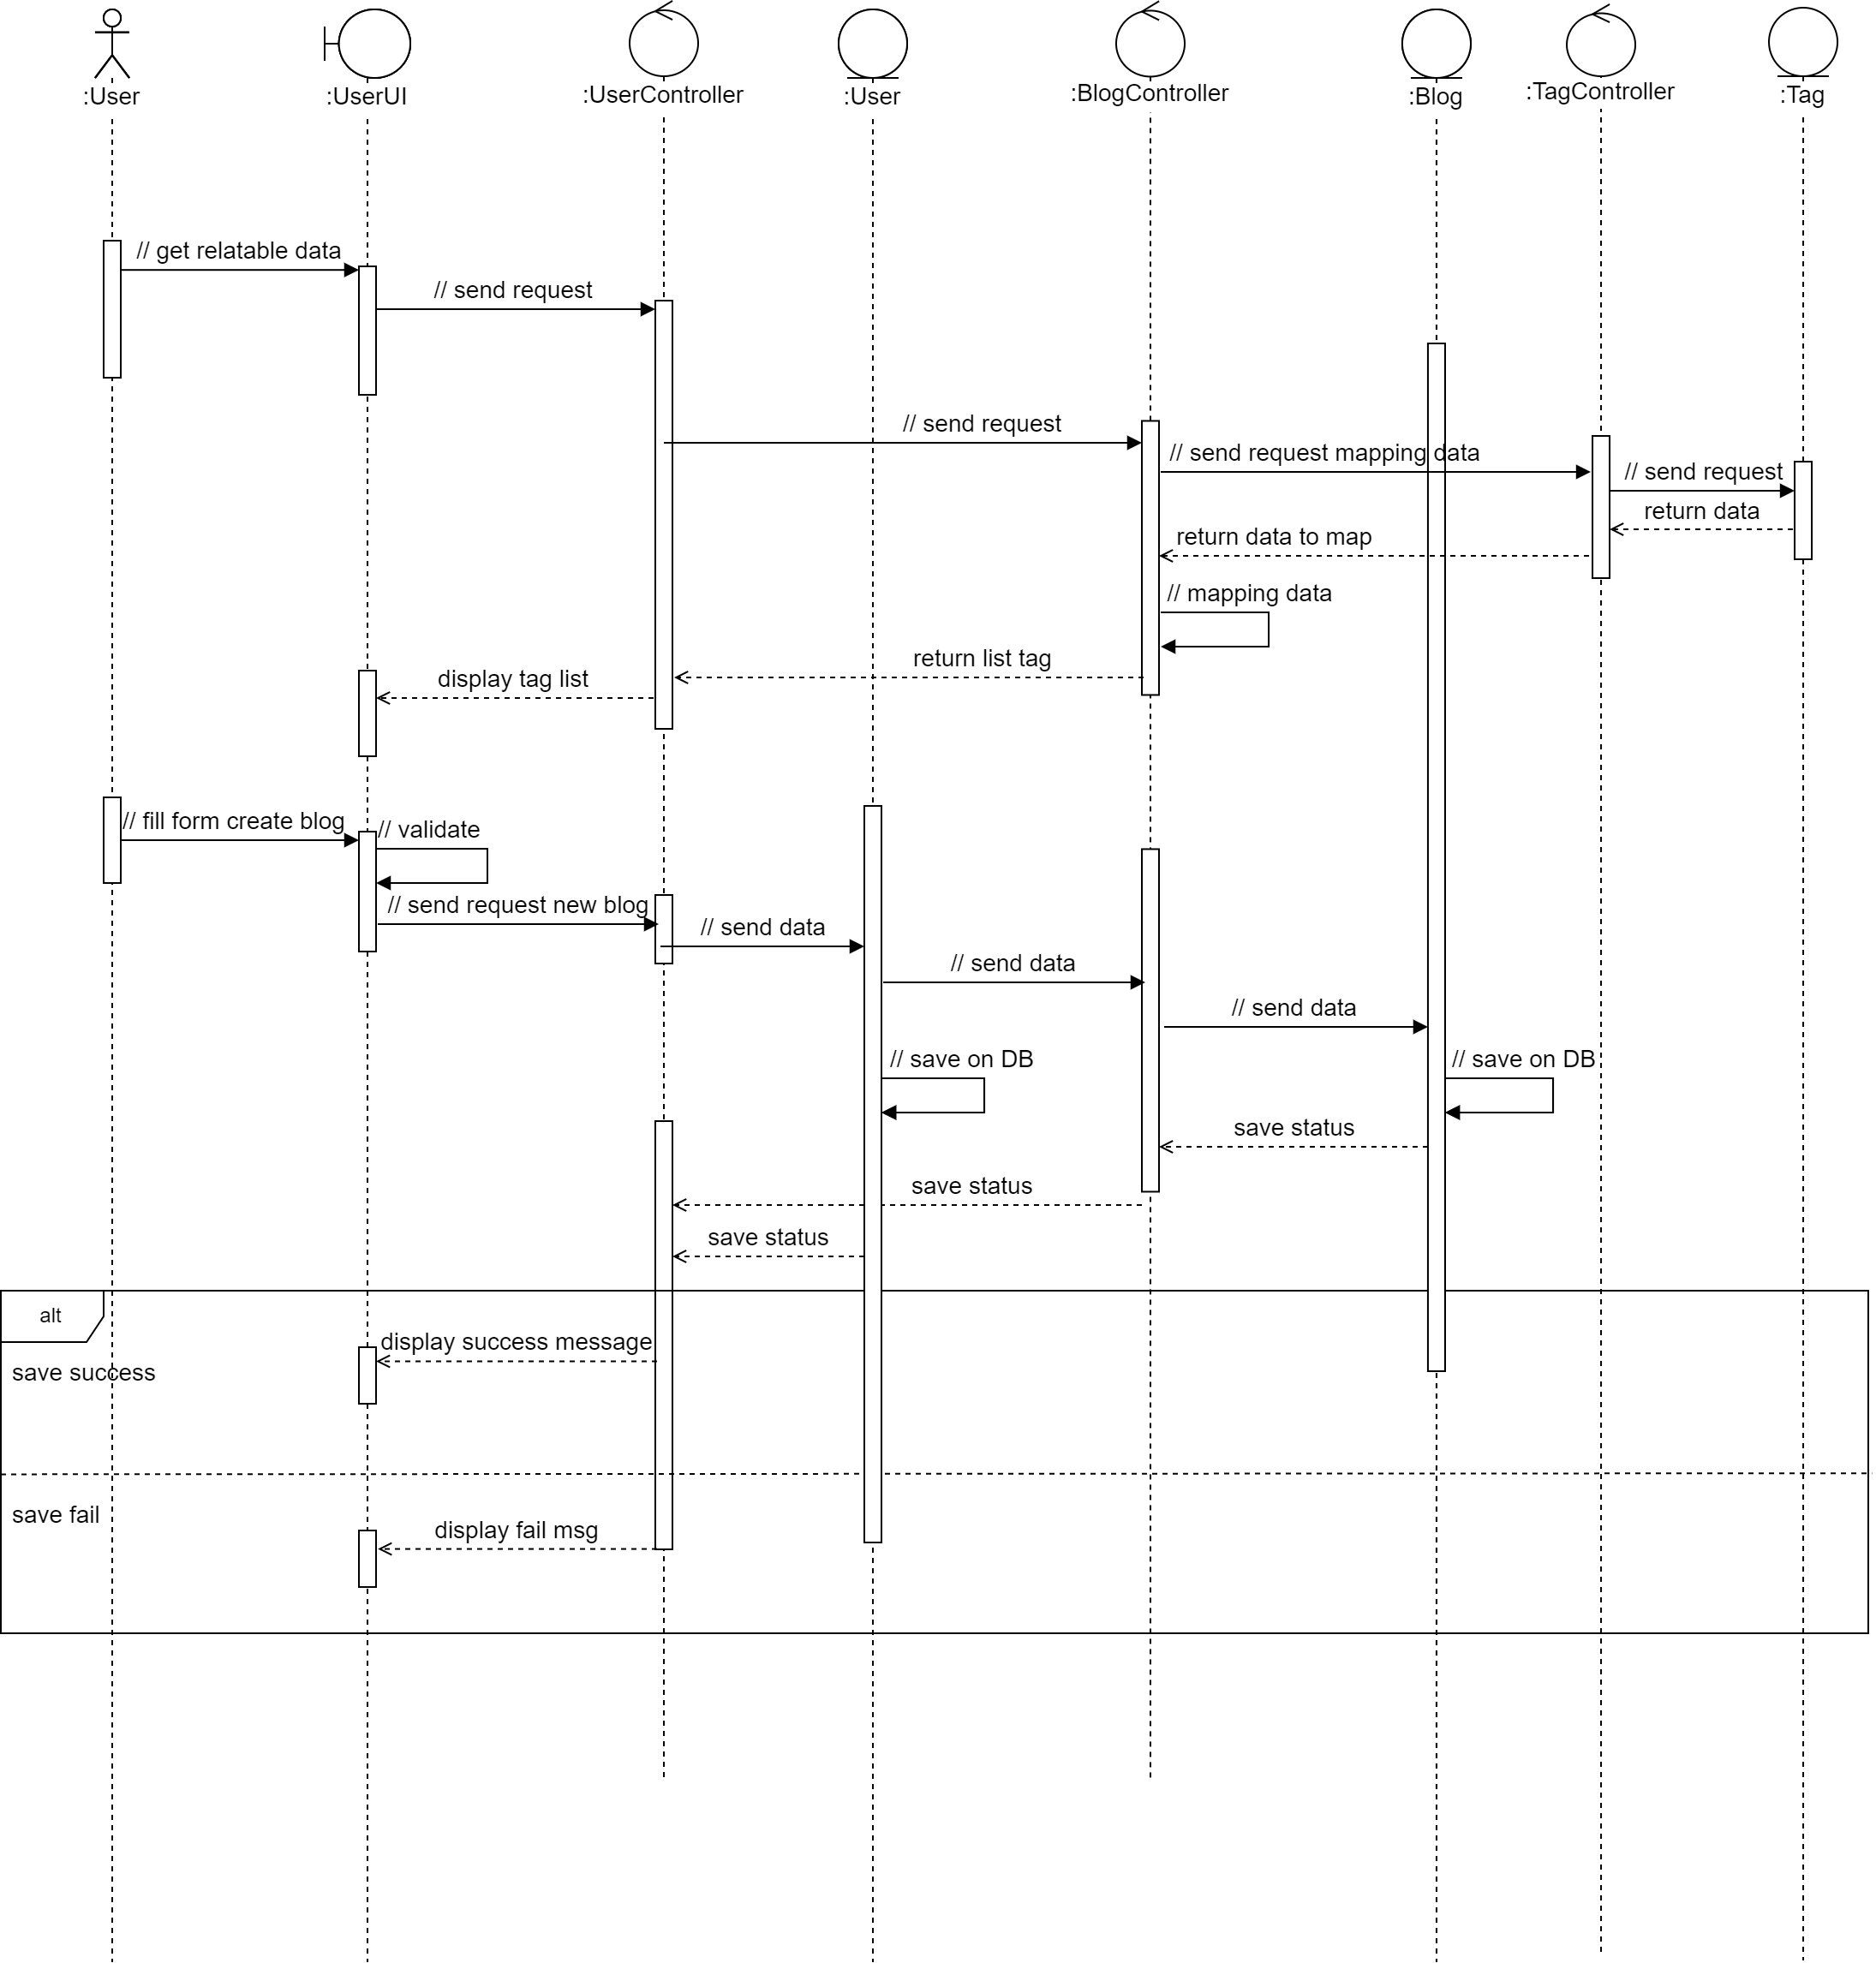
\includegraphics[width=\linewidth]{./img/uc15.png}
	\caption{Biểu đồ tuần tự - Ca sử dụng Tạo bài viết trên diễn đàn}
\end{figure}

\subsubsection{Các ca sử dụng quản lý của Quản trị viên}
\begin{figure}[H]
	\centering
	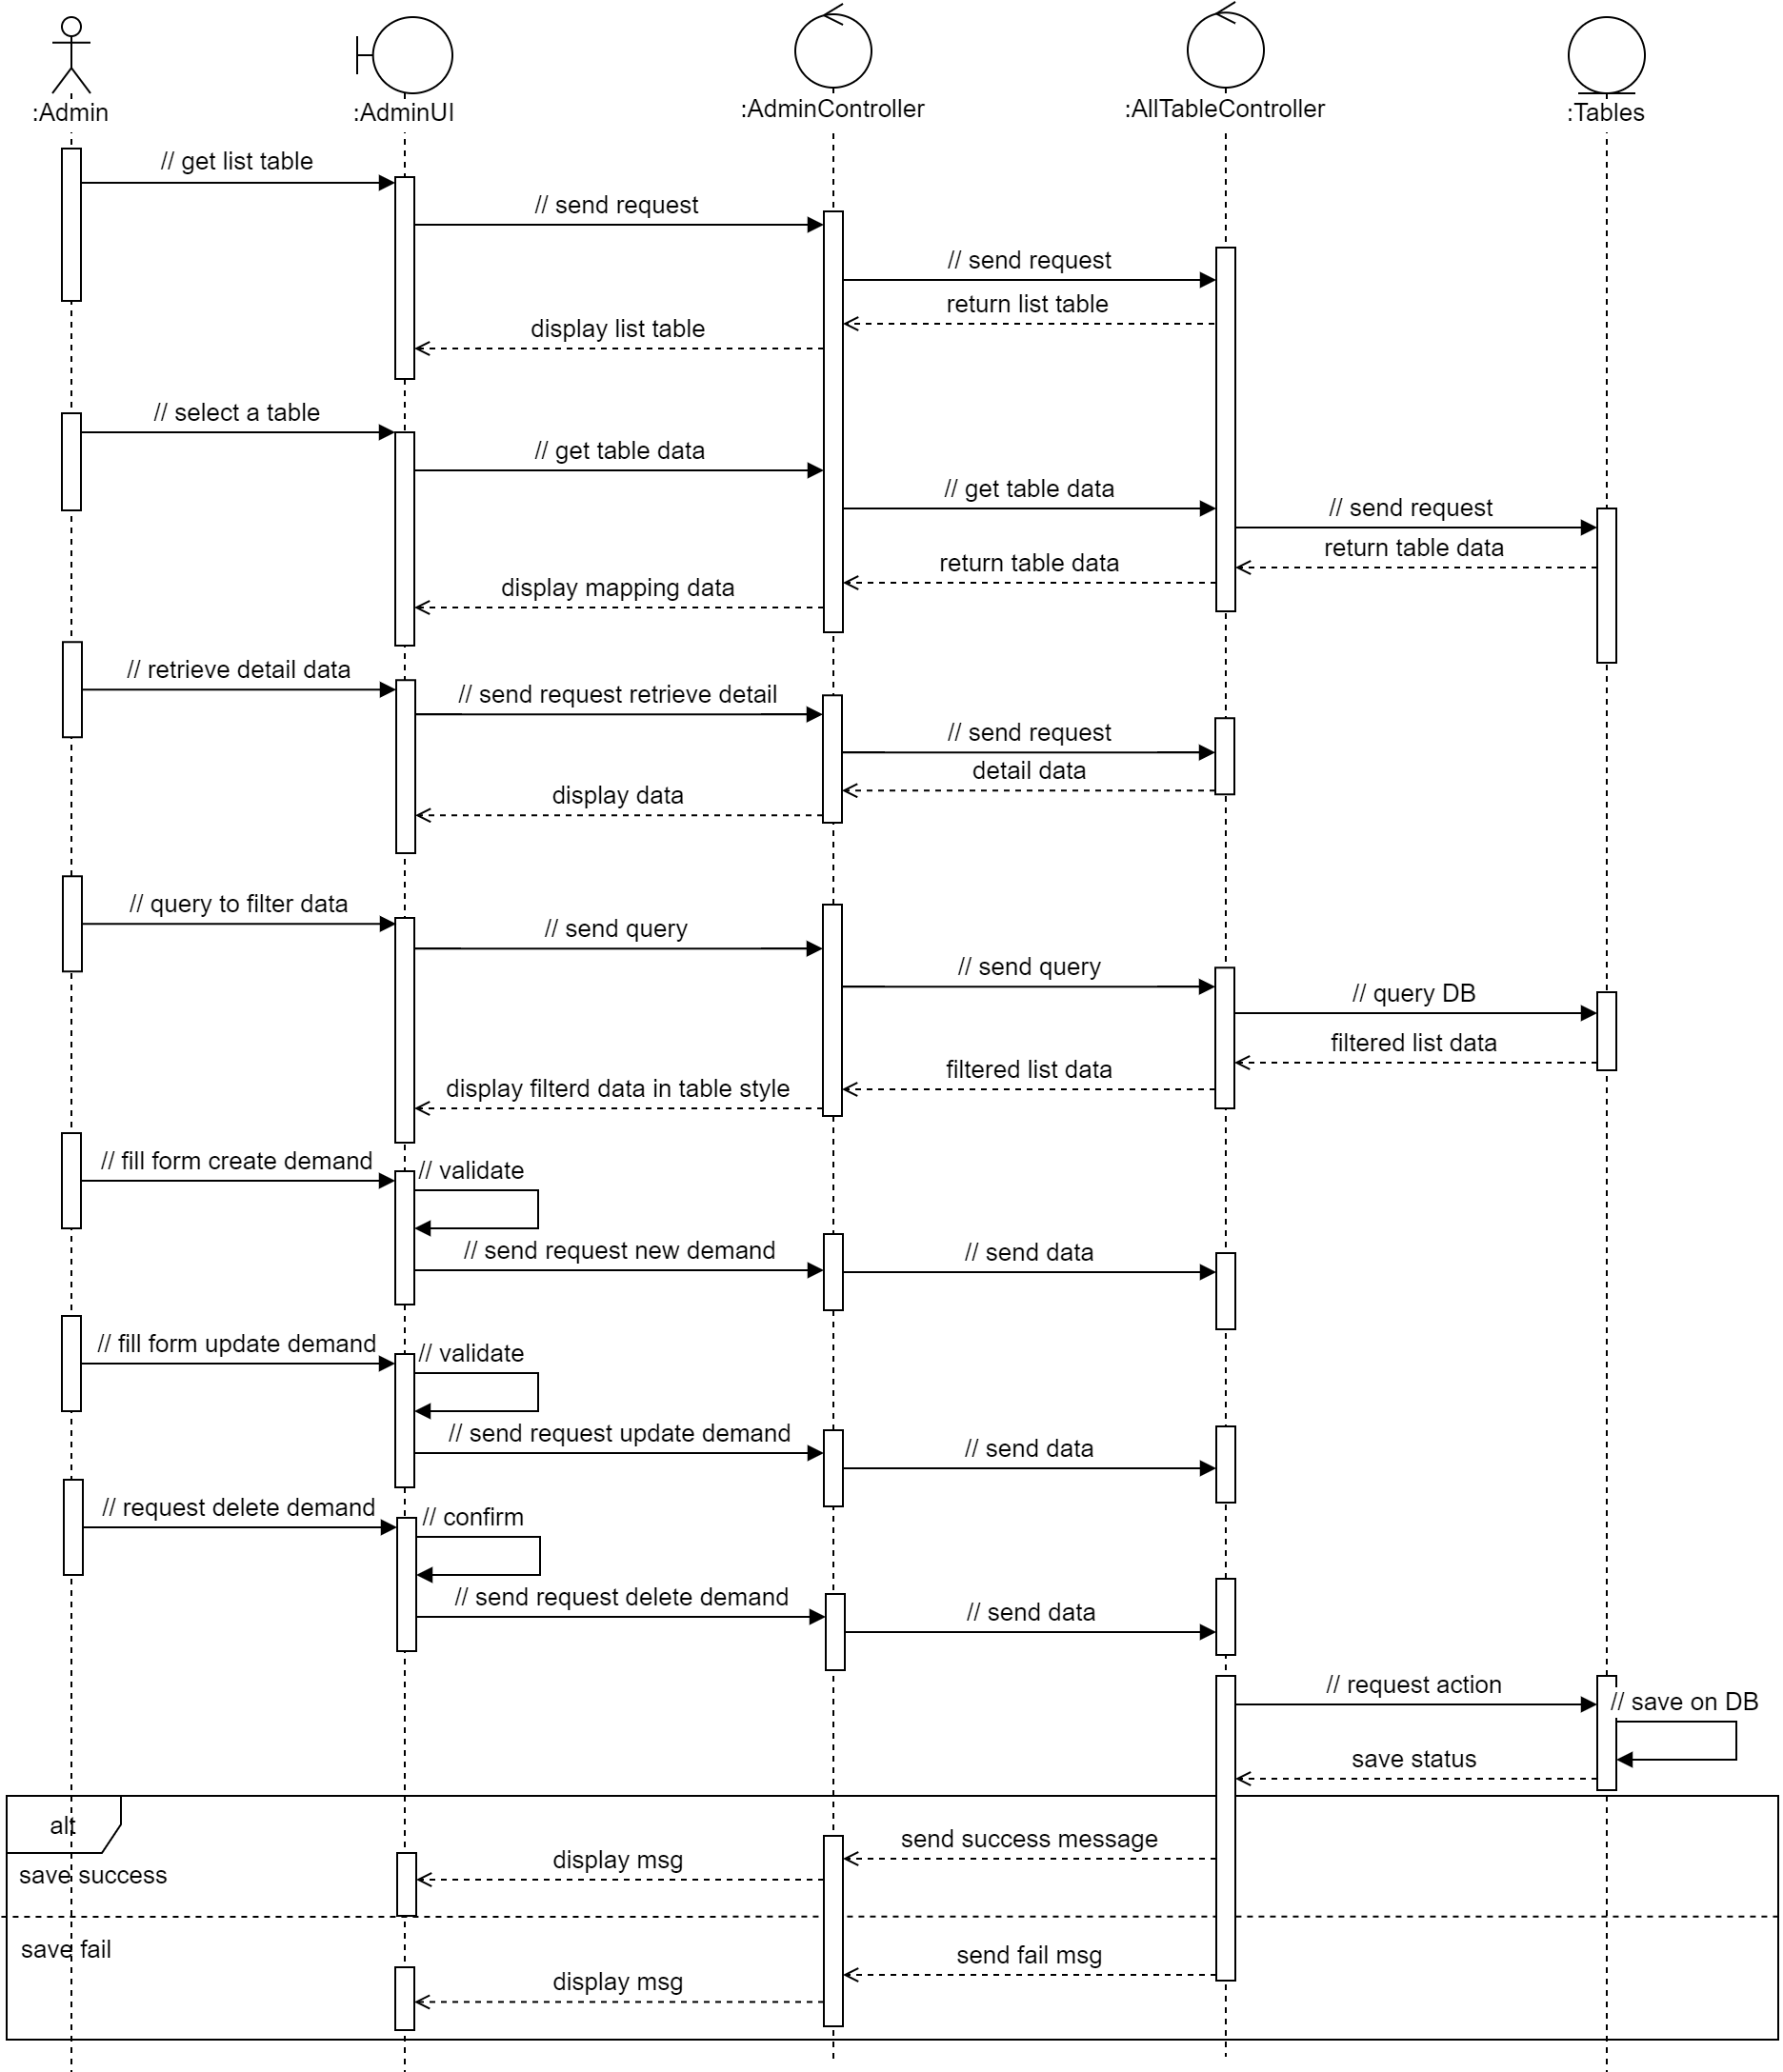
\includegraphics[width=\linewidth]{./img/uc16-19.png}
	\caption{Biểu đồ tuần tự - Các ca sử dụng quản lý của Quản trị viên}
\end{figure}

\subsubsection{Xác minh tài khoản mới}
\begin{figure}[H]
	\centering
	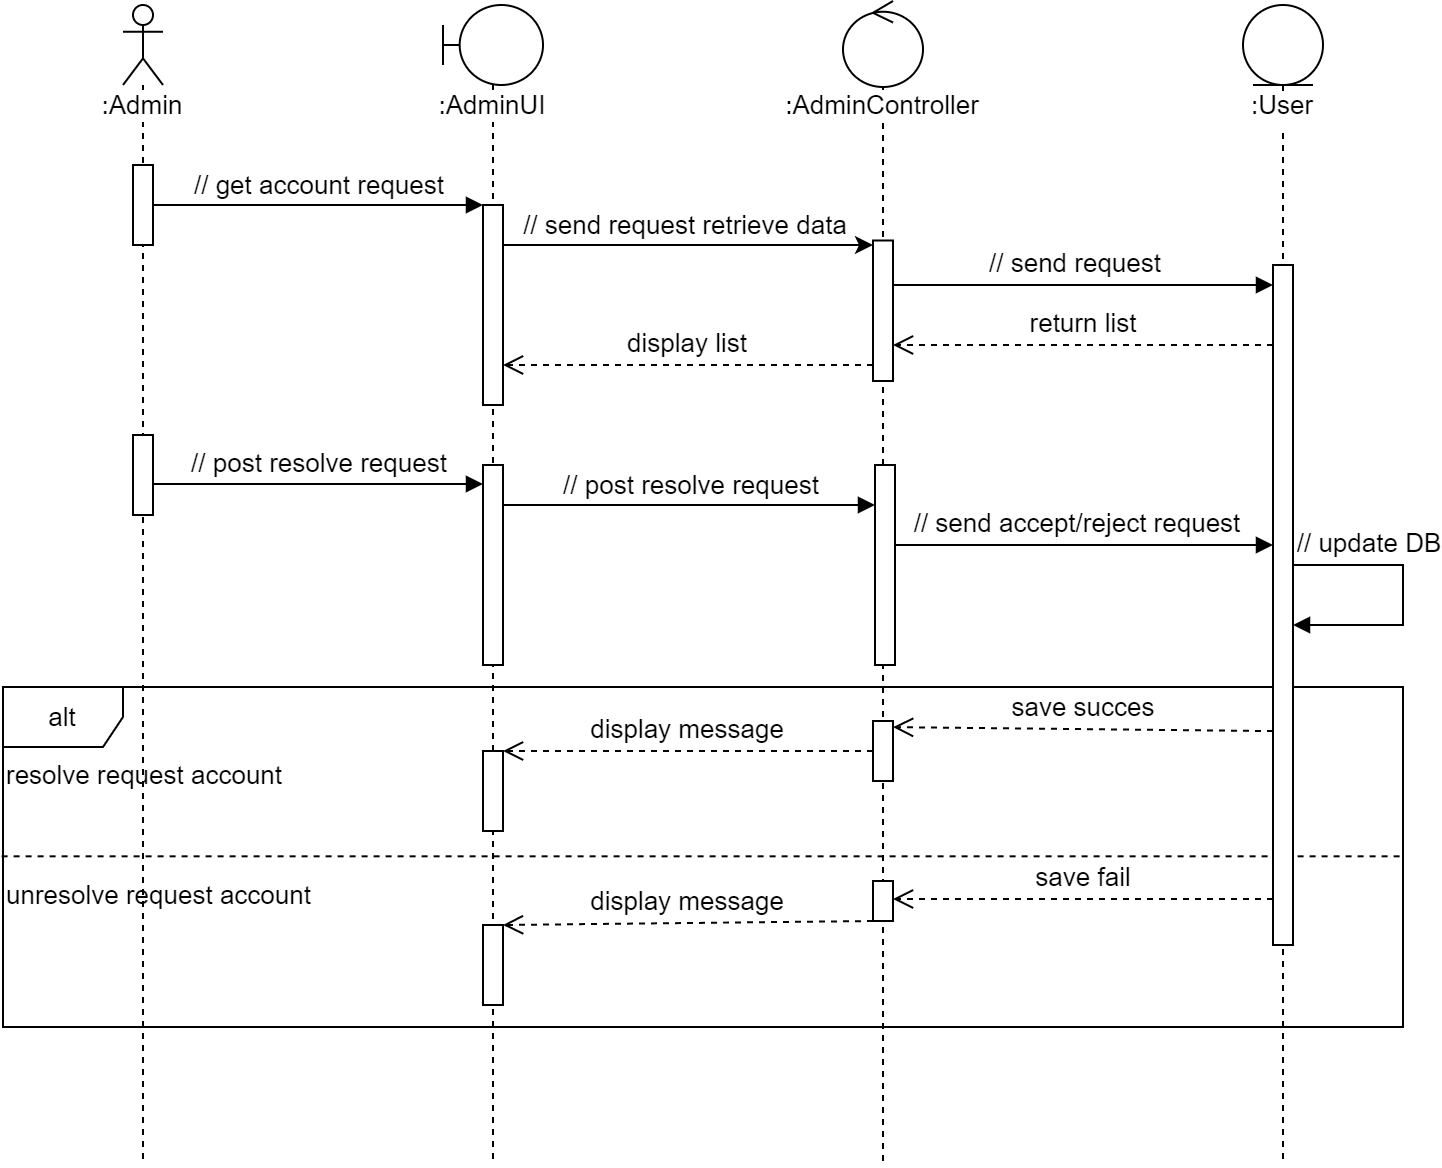
\includegraphics[width=\linewidth]{./img/uc20.png}
	\caption{Biểu đồ tuần tự - Ca sử dụng Xác minh tài khoản mới}
\end{figure}

Tài khoản do khách tạo có vai trò mặc định là chưa xác định. Để các tài khoản đó có thể truy cập vào hệ thống và thực hiện các chắc năng như của người dùng, quản trị viên cần cấp cho tài khoản quyền người dùng. Hay nói cách khác, bằng cách cấp tài khoản các vai trò tương ứng: người dùng, quản trị viên, khi đăng nhập vào hệ thống sẽ có các chức năng tương tự.

\subsubsection{Tạo người dùng hoặc quản trị viên mới}
\begin{figure}[H]
	\centering
	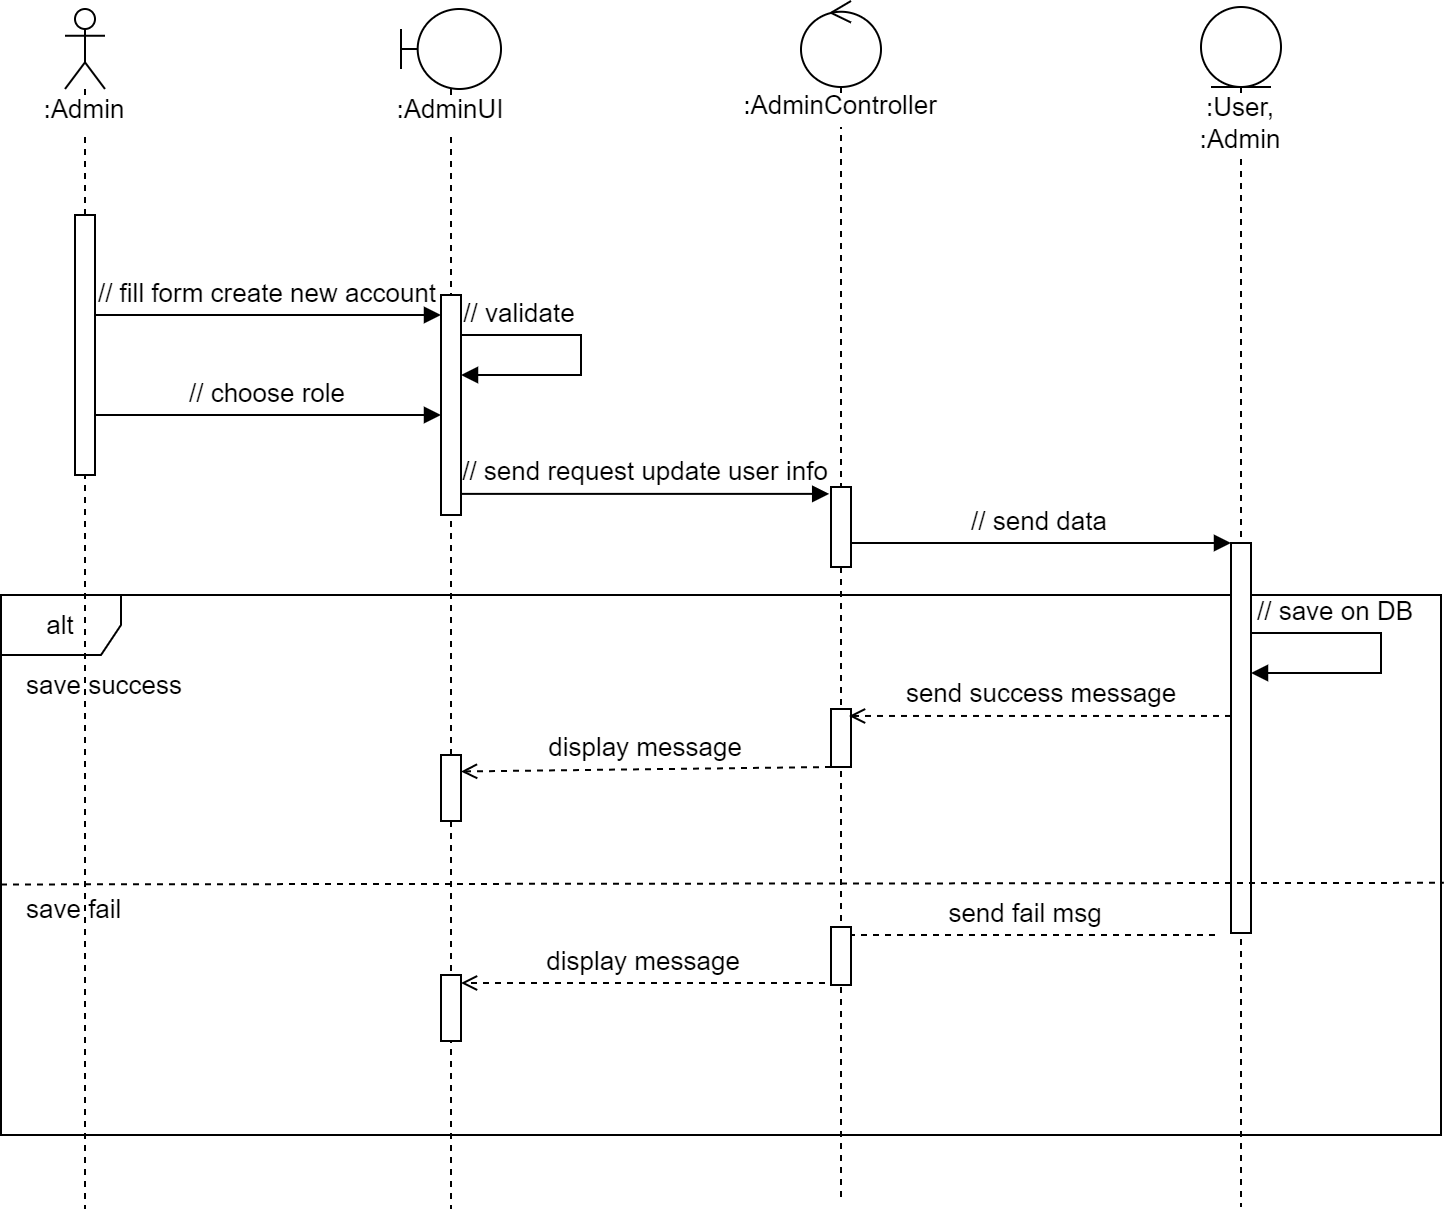
\includegraphics[width=\linewidth]{./img/uc21.png}
	\caption{Biểu đồ tuần tự - Ca sử dụng Tạo người dùng hoặc quản trị viên mới}
\end{figure}

Quản trị viên cũng có khả năng tạo tài khoản cho người dùng hoặc quản trị viên mới. Tài khoản được quản trị viên tạo sẽ không cần phải thông qua bước xác minh.

\end{document}

Hệ thống có 5 thành phần chính:
\begin{enumerate}
	\item Web Client: dành cho người dùng máy tính.
	\item Mobile App: dành cho người dùng di động.
	\item Server: Cung cấp API để client hiển thị.
	\item Cache Server: lưu trữ các dữ liệu được truy cập nhiều. Cụ thể, cache lưu lại các token bị blacklist.
	\item Database: lưu trữ thông tin về các thực thể trên hệ thống.
\end{enumerate}

\begin{figure}[H]
	\centering
	\includegraphics[width=\linewidth]{./images/high_level_diagram.png}
	\caption{Biểu đồ thiết kế bậc cao}
\end{figure}

\section{Thiết kế API}

API của hệ thống được thiết kế theo chuẩn REST để dễ dàng sử dụng. Tài liệu về API được lập trình viên backend tạo và upload lên \url{https://honyomi.stoplight.io/}.

\section{Thiết kế cơ sở dữ liệu}
Dù nhóm quyết định sử dụng cơ sở dữ liệu NoSQL dạng Document-base nhưng các lược đồ của cơ sở dữ liệu vẫn được nhóm xây dựng dựa trên mô hình thực thể - quan hệ (ER).
\begin{figure}[H]
	\centering
	\includegraphics[width=\linewidth]{./images/image8.png}
	\caption{Biểu đồ thiết kế cơ sở dữ liệu}
\end{figure}
Dựa vào phân tích ER trên, các lược đồ được sinh ra sẽ gồm các Document sau:
\begin{itemize}
	\item User: lưu thông tin và cài đặt của người dùng.
	\item History: lưu lịch sử đọc truyện của người dùng.
	\item Favorite: lưu danh sách yêu thích của người dùng.
	\item Manga: lưu danh sách truyện trên hệ thống.
	\item Chapter: lưu danh sách chương truyện.
	\item Category: lưu thể loại truyên.
	\item Author: lưu danh sách tác giả.
\end{itemize}
